\chapter{Scalable Learning of Probabilistic Circuits}
\label{ch:scalable}

Considering the many benefits and drawbacks of the current state-of-the-art learning algorithms
addressed in \Cref{ch:learning}, and emphasizing the need for scalability and accessibility, we now
present the main contributions of this dissertation, proposing two novel structure learning
algorithms for probabilistic circuits. We approach the problem of learning scalable PCs from two
distinct points of view. In \Cref{sec:logical}, we are interested in PCs whose support encodes a
given logical constraint as certain knowledge; we show how both the probabilistic issue of data
fitness, as well as the logical question of whether the circuit successfully compiles a knowledge
base can be accomplished by aggregating PC samples into ensembles of models. In \Cref{sec:data}, we
look at PCs solely from the perspective of data fitness; we exploit the connection between PCs and
generative random forests \citep{correia20,ho95} and revisit a well-known technique based on random
projections for constructing random trees \citep{dasgupta08a,dasgupta08b}, presenting a simple and
fast yet effective way of learning PCs.

The contents of \Cref{sec:logical} come from our contributions in \citet{geh21a}, while
\Cref{sec:data} comes, in part, from \citet{geh21b}.

\section{A Logical Perspective}
\label{sec:logical}

\Cref{rem:initpc} briefly mentioned the question of compiling logical constraints into smooth,
structure decomposable and deterministic logic circuits (i.e.\ (P)SDDs \cite{darwiche11,kisa14}).
Indeed, although there are many existing approaches to learning circuits from logical formulae,
most are only useful for specific tasks \citep{choi16,choi15,shen17,choi17}. Although there are
more generalistic ways of producing circuits, namely from CNFs and DNFs \citep{oztok15,choi13};
logic formulae which incorporate more complex relationships such as cardinality constraints either
have no tractable representation \citep{nishino16} or require the addition of latent variables
\citep{sinz05}. More importantly, because variables which do not play a role in the logical
formulae are completely discarded in the compilation process, translating these \emph{logic}
circuits into \emph{probabilistic} circuits involves naïve assumptions on the discarded variables,
such as fully factorizing them.

Surprisingly, to our knowledge there have been next to no work on learning the structure of PCs
from scratch by looking at both logical formulae \emph{and} data. Even worse, the couple that do
are restricted to very preliminary work: \citet{mattei19} came up with a \divclass{} prototype for
a top-down approach to sampling a special class of PSDDs whose primes are conjunctions of literals
in a similar manner to \textproc{XPC}s, proposing a Bayesian information criterion to searching the
sample space, yet no practical algorithm was fully formulated; \citet{geh20} expanded on
\citeauthor{mattei19}'s work by formalizing an algorithm and introducing a BDD to guide sampling,
however the generated circuits suffered from an exponential blow-up in size.

In this section, we propose a solution inspired by \citet{geh20,mattei19}, yet without the
previously mentioned problems that come with them. In summary, we propose a sampling procedure to
efficiently generating PSDDs whose primes are always conjunctions of literals; to overcome the
exponential blow-up, these PSDDs only partially encode their prior logical restrictions. To
diversify sampling, local transformations similar in spirit to \incrclass{} algorithms are used.
Of worth, we found that not only is this process incredibly fast even under intricate logical
formulae, but by combining samples into an ensemble we achieve competitive results against the
state-of-the-art.

Before we address our contributions, we should first fix some notation on the issue of
propositional logic. We treat propositional variables as 0/1-valued random variables and use them
interchangeably. Given a Boolean formula, we write $\langle f\rangle$ to denote its semantics,
i.e.\ the Boolean function represented by $f$. For Boolean formulas $f$ and $g$, we write $f\equiv
g$ if they are logically equivalent, i.e.\ if $\langle f\rangle=\langle g\rangle$; we abuse
notation and write $\phi\equiv f$ to indicate that $\phi=\langle f\rangle$ for a Boolean function
$\phi$. We overload the scope function once again for logical formulae: $\Sc(f)$ denotes the set of
variables that appear in $f$.

Because we are only interested in smooth, structure decomposable and deterministic PCs whose
support is defined by a logical formula, we shall adopt the usual notation of PSDDs, which we
present next.

\begin{definition}[Partition]\label{def:partition}
  Let $\phi(\set{x},\set{y})$ be a Boolean function over disjoint sets of variables $\set{X}$ and
  $\set{Y}$, and $\mathcal{D}=\{(p_i,s_i)\}_{i=1}^k$ be a set of tuples where $p_i$ (the prime) and
  $s_i$ (the sub) are formulae over $\set{X}$ and $\set{Y}$ respectively, satisfying $p_i\wedge
  p_j\equiv\bot$ for each $i\neq j$ and $\bigvee_{i=1}^k p_i\equiv\top$. We say that $\mathcal{D}$
  is an ($\set{X}$, $\set{Y}$)-partition of $\phi$ if and only if
  $\phi\equiv\bigvee_{i=1}^k(p_i\wedge s_i)$.
\end{definition}

An (exact) partition\footnote{The naming \emph{partition} is unfortunate. The nomenclature in
probabilistic circuits is full of many other partitions, either using the term to conjure meaning
from set theory when dealing with data splits (see \Cref{sec:divconq}), partition nodes in region
graphs (see \Cref{sec:random}) or in PSDD literature in this section. Here (and only here),
partitions will mean stricly the latter.} is no more than a smooth, structure decomposable and
deterministic circuit rooted at a sum (or disjunction) node whose children are products (or
conjunctions); the primes of these products must necessarily be mutual exclusive (formally,
$p_i\wedge p_j\equiv\bot$) and exhaustive (formally, $\bigvee_{i=1}^k p_i\equiv\top$).
Semantically, a partition states that a logical formula decomposes into $k$ exact conjunctions of
pairs of prime and sub. The \protect\tikz\protect\draw[very thick,dashed,pbrickred] (0,0) rectangle
(0.5,-0.25); box in \Cref{fig:psdd} shows a partition whose primes are $\textcolor{pviolet}{p_1}=A$
and $\textcolor{pviolet}{p_2}=\neg A$, and subs are $\textcolor{psandy}{s_1}=\neg B$ (represented
as a PC rooted at \protect\tikz\protect\newNamedOrNode[scale=0.8,baseline=-0.75ex,fill=boxolive]{r}{0,0}{2};)
and $\textcolor{psandy}{s_2}=\neg C$ (represented as the PC rooted at
\protect\tikz\protect\newNamedOrNode[scale=0.8,baseline=-0.75ex,fill=boxmunsel]{r}{0,0}{2};).
Recall that the conjunction between a prime and sub is called an \emph{element}, here shown as
\inode[fill=boxpink!80]{\newAndNode} and \inode[fill=boxred]{\newAndNode}.

\begin{figure}[t]
  \begin{tikzpicture}
    \node (tab) at (-7,-0.5) {
      \begin{tabular}{|ccc|c|} \hline
        $A$ & $B$ & $C$ & $p(\set{x})$\\
        \hline
        0 & 0 & 0 & 0.1\\
        0 & 1 & 0 & 0.1\\
        1 & 0 & 0 & 0.2\\
        1 & 0 & 1 & 0.6\\
        \hline
      \end{tabular}
    };

    \node at ($(tab) + (0,-2)$) {\small$\phi(A,B,C)=(A\to\neg B)\wedge(C\to A)$};

    \newVtreeNode{v_root}{$(tab) + (0,-3)$}{1};
    \newVtreeNode[fill=boxorange!80]{v_lr}{$(v_root)+(-0.55, -1.5)$}{$A$};
    \newVtreeNode{v_rr}{$(v_root)+(0.55,-1.5)$}{2};
    \newVtreeNode[fill=boxblue!50]{v_lrr}{$(v_root)+(0,-3.0)$}{$B$};
    \newVtreeNode[fill=boxgoldenrod!70]{v_rrr}{$(v_root)+(1.1, -3.0)$}{$C$};
    \draw (v_root) -- (v_lr);
    \draw (v_root) -- (v_rr);
    \draw (v_rr) -- (v_lrr);
    \draw (v_rr) -- (v_rrr);

    \newNamedOrNode[fill=boxgreen,inputs=nn]{r}{0,0}{1};
    \newAndNode[fill=boxpink!80,inputs=nn]{p1}{$(r) + (-0.75,-1.5)$};
    \newAndNode[fill=boxred,inputs=nn]{p2}{$(r) + (0.75,-1.5)$};
    \newNamedOrNode[fill=boxolive,inputs=nn]{s1}{$(p1.input 2) + (0,-1.0)$}{2};
    \newNamedOrNode[fill=boxmunsel,inputs=nn]{s2}{$(p2.input 2) + (2.2,-1.0)$}{2};
    \newAndNode[inputs=nn]{s1p1}{$(r) + (-1.5,-4.25)$};
    \newAndNode[inputs=nn]{s2p1}{$(r) + (2.1,-4.5)$};
    \newAndNode[inputs=nn]{s2p2}{$(r) + (3.9,-4.5)$};
    \newOrNode[inputs=nn]{s3}{$(r) + (-0.25,-5.5)$};

    \node[fill=boxorange!80,minimum size=17pt,label=center:{$A$}] (p1l) at ($(p1.input 1) + (-0.75,-1.0)$) {};
    \node[fill=boxorange!80,minimum size=17pt,label=center:{$\neg A$}] (p2l) at ($(p2.input 1) + (0.0,-1.0)$) {};
    \node[fill=boxblue!50,minimum size=17pt,label=center:{$\neg B$}] (s1p1l) at ($(s1p1.input 1) + (-0.75,-0.75)$) {};
    \node[fill=boxblue!50,minimum size=17pt,label=center:{$\neg B$}] (s2p1l1) at ($(s2p1.input 1) + (-0.5,-1.0)$) {};
    \node[fill=boxgoldenrod!70,minimum size=17pt,label=center:{$\neg C$}] (s2p1l2) at ($(s2p1.input 2) + (0.5,-1.0)$) {};
    \node[fill=boxblue!50,minimum size=17pt,label=center:{$B$}] (s2p2l1) at ($(s2p2.input 1) + (-0.5,-1.0)$) {};
    \node[fill=boxgoldenrod!70,minimum size=17pt,label=center:{$\neg C$}] (s2p2l2) at ($(s2p2.input 2) + (0.5,-1.0)$) {};
    \node[fill=boxgoldenrod!70,minimum size=17pt,label=center:{$C$}] (s3l1) at ($(s3.input 1) + (-0.5,-1.0)$) {};
    \node[fill=boxgoldenrod!70,minimum size=17pt,label=center:{$\neg C$}] (s3l2) at ($(s3.input 2) + (0.5,-1.0)$) {};

    \draw[edge] (r.input 1) -- ++(0,-0.4) -| node[above left]{\color{pdgreen}$.8$} (p1.east);
    \draw[edge] (r.input 2) -- ++(0,-0.4) -| node[above right]{\color{pdgreen}$.2$} (p2.east);
    \draw[edge] (p1.input 1) -- ++(0,-0.4) -| (p1l.north);
    \draw[edge] (p2.input 1) -- ++(0,-0.4) -| (p2l.north);
    \draw[edge] (s1p1.input 1) -- ++(0,-0.2) -| (s1p1l.north);
    \draw[edge] (s2p1.input 1) -- ++(0,-0.4) -| (s2p1l1.north);
    \draw[edge] (s2p1.input 2) -- ++(0,-0.4) -| (s2p1l2.north);
    \draw[edge] (s2p2.input 1) -- ++(0,-0.4) -| (s2p2l1.north);
    \draw[edge] (s2p2.input 2) -- ++(0,-0.4) -| (s2p2l2.north);
    \draw[edge] (s3.input 1) -- ++(0,-0.4) -| node[above left]{\color{pdgreen}$.75$} (s3l1.north);
    \draw[edge] (s3.input 2) -- ++(0,-0.4) -| node[above right]{\color{pdgreen}$.25$} (s3l2.north);
    \draw[edge] (p1.input 2) -- ++(0,-0.4) -| (s1.east);
    \draw[edge] (p2.input 2) -- ++(0,-0.4) -| (s2.east);
    \draw[edge] (s1.west) -- ++(0,-0.3) node[below right]{\color{pdgreen}$1.0$} -| (s1p1.east);
    \draw[edge] (s2.input 1) -- ++(0,-0.4) -| node[above left]{\color{pdgreen}$.5$} (s2p1.east);
    \draw[edge] (s2.input 2) -- ++(0,-0.4) -| node[above right]{\color{pdgreen}$.5$} (s2p2.east);
    \draw[edge] (s1p1.input 2) -- ++ (0,-0.2) -| (s3.east);

    \draw[very thick,dashed,pbrickred] ($(p1l) + (-1.0,3.5)$) rectangle ($(s2) + (1.5,-1)$);
    \node at ($(p1l) + (-0.75,0)$) {\color{pviolet}$p_1$};
    \node at ($(s1) + (0.5,0.5)$) {\color{psandy}$s_1$};
    \node at ($(p2l) + (0.75,0)$) {\color{pviolet}$p_2$};
    \node at ($(s2) + (0.5,0.5)$) {\color{psandy}$s_2$};
  \end{tikzpicture}
  \caption{A PSDD encoding the logical constraint $\phi(A,B,C)=(A\to\neg B)\wedge(C\to A)$,
  following the distribution set by the probability table on the top left corner and whose
  structure is defined by the vtree pictured on the bottom left corner.}
  \label{fig:psdd}
\end{figure}

\subsection{\textproc{SamplePSDD}}
\label{subsection:samplepsdd}

We now describe how to efficiently learn PSDDs by sampling and averaging. The procedure takes
inspiration from \divclass{} algorithms in the sense that we construct a PSDD structure top-down by
recursively decomposing a logical formula (instead of data). At the same time, we employ local
transformations similar to \incrclass{} approaches on a partially constructed circuit to diversify
samples. All this procedure is done randomly in a similar fashion to \textproc{XPC}s, where we
restrict primes to be random conjunctions of literals and sample variables according to a
previously learned or randomly sampled vtree. To better understand how this is done, we must first
consider a naïve approach.

\begin{figure}[t]
  \begin{tikzpicture}
    \node at (0,1.0) {\normalsize$\phi(A,B,C,D)=(A\wedge\neg B\wedge\neg D)\vee(B\wedge\neg C\wedge D)$};

    \newNamedOrNode[fill=boxgreen,inputs=nnnn]{r}{0,0}{1};
    \newNamedAndNode[fill=boxblue,inputs=nn]{a1}{$(r) + (-3.0,-1.5)$}{$e_1$};
    \newNamedAndNode[fill=boxorange,inputs=nn]{a2}{$(r) + (-1.0,-1.5)$}{$e_2$};
    \newNamedAndNode[fill=boxred,inputs=nn]{a3}{$(r) + (1.0,-1.5)$}{$e_3$};
    \newNamedAndNode[fill=boxgoldenrod,inputs=nn]{a4}{$(r) + (3.0,-1.5)$}{$e_4$};

    \node (p1) at ($(a1.input 1) + (-0.6,-0.75)$) {\color{pviolet}$A\wedge B$};
    \node (p2) at ($(a2.input 1) + (-0.6,-0.75)$) {\color{pviolet}$A\wedge\neg B$};
    \node (p3) at ($(a3.input 1) + (-0.6,-0.75)$) {\color{pviolet}$\neg A\wedge B$};
    \node (p4) at ($(a4.input 1) + (-0.7,-0.75)$) {\color{pviolet}$\neg A\wedge\neg B$};
    \node (s1) at ($(a1.input 2) + (0,-1.25)$) {\color{psandy}$\neg C\wedge D$};
    \node (s2) at ($(a2.input 2) + (0,-1.25)$) {\color{psandy}$\neg D$};
    \node (s3) at ($(a3.input 2) + (0,-1.25)$) {\color{psandy}$\neg C\wedge D$};
    \node (s4) at ($(a4.input 2) + (0,-1.25)$) {\color{psandy}$\bot$};
    \node at ($(r) + (3,0.25)$) {\large$\textcolor{psandy}{s_i}=\phi|_{\textcolor{pviolet}{p_i}}$};

    \draw[edge] (r.input 1) -- ++(0,-0.2) -| (a1);
    \draw[edge] (r.input 2) -- ++(0,-0.4) -| (a2);
    \draw[edge] (r.input 3) -- ++(0,-0.4) -| (a3);
    \draw[edge] (r.input 4) -- ++(0,-0.2) -| (a4);
    \draw[edge] (a1.input 1) -- ++(0,-0.3) -| (p1);
    \draw[edge] (a2.input 1) -- ++(0,-0.3) -| (p2);
    \draw[edge] (a3.input 1) -- ++(0,-0.3) -| (p3);
    \draw[edge] (a4.input 1) -- ++(0,-0.3) -| (p4);
    \draw[edge] (a1.input 2) -- ++(0,-0.4) -| (s1);
    \draw[edge] (a2.input 2) -- ++(0,-0.4) -| (s2);
    \draw[edge] (a3.input 2) -- ++(0,-0.4) -| (s3);
    \draw[edge] (a4.input 2) -- ++(0,-0.4) -| (s4);

    \newVtreeNode{root}{6.5,1.0}{1};
    \newVtreeNode{nr}{$(root) + (-1.0,-1.25)$}{2};
    \newVtreeNode{n1}{$(root) + (1.0,-1.25)$}{3};
    \newVtreeNode{n2}{$(nr) + (-0.5,-1.25)$}{$A$};
    \newVtreeNode{ne}{$(nr) + (0.5,-1.25)$}{$B$};
    \newVtreeNode{n3}{$(n1) + (-0.5,-1.25)$}{4};
    \newVtreeNode{n4}{$(n1) + (0.5,-1.25)$}{$C$};
    \newVtreeNode{n5}{$(n3) + (-0.5,-1.25)$}{$D$};
    \newVtreeNode{n6}{$(n3) + (0.5,-1.25)$}{$E$};
    \draw (root) -- (n1);
    \draw (n1) -- (n3);
    \draw (root) -- (nr);
    \draw (nr) -- (n2);
    \draw (nr) -- (ne);
    \draw (n1) -- (n3);
    \draw (n1) -- (n4);
    \draw (n3) -- (n6);
    \draw (n3) -- (n5);
  \end{tikzpicture}
  \caption{A(n exact) partition of $\phi$ where we assume that primes are conjunctions of literals.
  Primes must be exhaustive, mutually exclusive, and have to follow the vtree's scope, here
  $\Sc(1^\gets)=\{A,B\}$. The subs are then the restriction of $\phi$ under the assignment induced
  by the primes.}
  \label{fig:partition}
\end{figure}

Let $\phi$ a logical formula acting as our knowledge base, and assume that a vtree $\vtree$ is
given beforehand. To compile a PSDD from $\phi$, we must decompose it down to a disjunction of
prime and sub conjunctions. This is a non-trivial problem, as primes must not only be mutual
exclusive (to ensure determinism) but exhaustive (to make sure the circuit is coherent with $\phi$
in all possible assignments). If we assume primes to be conjunctions of literals, then to adhere to
\Cref{def:partition} there must be an exponential number of elements $2^{|\Sc(v^\gets)|}$, where
$v$ is the vtree node that corresponds to the partition. Subs, however, are easy to retrieve as
they correspond to the restriction of $\phi$ under the assignment induced by the prime.
\Cref{fig:partition} shows a partition whose primes are conjunctions over $A$ and $B$. This problem
is the same as the one faced by \citet{geh20}: under the assumption of conjunctions of literals as
primes, $\phi$ can only be faithfully represented as a PSDD if the circuit is exponential.

To overcome this exponential blow-up, we might restrict the number of primes at each partition.
Unfortunately, if we bound this number to a constant, say $k$, and randomly sample primes from the
space of all possible conjunctions of literals, then we face yet another problem: the scope of subs
might contain variables not in their corresponding vtree node. Take the top circuit in
\Cref{fig:partial} as an example. Note that the scope for primes is defined by
$\Sc(1^\gets)=\{A,B,C\}$, with $\Sc(1^\to)=\{D,E\}$ for subs; so sampled primes $p_1=A\wedge B$,
$p_2=A\wedge\neg B$ and $p_3=\neg A$ must come from $\Sc(1^\gets)$. However, because
$s_1=\phi|p_1=\neg C\wedge D$ and $s_3=\phi|p_3=B\wedge\neg C \wedge D$, meaning that
$\Sc(s_1)\not\subseteq\Sc(1^\to)$ and $\Sc(s_3)\not\subseteq\Sc(1^\to)$, subs violate the
factorization imposed by the vtree $\mathcal{V}$, making the circuit non-structure decomposable
(albeit decomposable). Here, we point out that the scope of the formula needs to be a subset of the
scope of its corresponding vtree for the PC to be structure decomposable, and not necessarily
the set itself, as variables that do not appear in the formula yet are part of the vtree's scope
play a \emph{probabilistic} role in the PSDD.

For these circuits to both preserve structure decomposability \emph{and} have tractable
representation, we need to resort to a weaker definition of a partition that relaxes the logical
constraints.

\begin{definition}[Partial partition]\label{def:partialpart}
  Let $\phi(\set{x},\set{y})$ be a Boolean function over disjoint sets of variables $\set{X}$ and
  $\set{Y}$, and $\mathcal{D}=\{(p_i,s_i)\}_{i=1}^k$ be a set of tuples where $p_i$ (the prime) and
  and $s_i$ (the sub) are formulae over $\set{X}$ and $\set{Y}$ respectively, satisfying $p_i\wedge
  p_j\equiv\bot$ for each $i\neq j$ and $\bigvee_{i=1}^k p_i\equiv\top$. We say that $\mathcal{D}$
  is a partial partition of $\phi$ if
  \begin{equation*}
    \left\langle\bigvee_{i=1}^k (p_i\wedge s_i)\right\rangle\geq\phi,
  \end{equation*}
  where the inequality is taken coordinate-wise.
\end{definition}

\begin{figure}[t]
  \begin{subfigure}[t]{\textwidth}
    \centering
    \begin{tikzpicture}[tips=proper]
      \node at (-2,1.0) {\normalsize$\phi(A,B,C,D)=(A\wedge\neg B\wedge\neg D)\vee(B\wedge\neg C\wedge D)$};

      \newNamedOrNode[fill=boxgreen,inputs=nnn]{r}{-2.35,0}{1};
      \newNamedAndNode[fill=boxblue,inputs=nn]{a1}{$(r) + (-2.0,-1.5)$}{$e_1$};
      \newNamedAndNode[fill=boxorange,inputs=nn]{a2}{$(r) + (0.0,-1.5)$}{$e_2$};
      \newNamedAndNode[fill=boxpink!80,inputs=nn]{a3}{$(r) + (2.0,-1.5)$}{$e_3$};

      \node (p1) at ($(a1.input 1) + (-0.6,-0.75)$) {\color{pviolet}$A\wedge B$};
      \node (p2) at ($(a2.input 1) + (-0.6,-0.75)$) {\color{pviolet}$A\wedge\neg B$};
      \node (p3) at ($(a3.input 1) + (-0.7,-0.75)$) {\color{pviolet}$\neg A$};
      \node (s1) at ($(a1.input 2) + (0,-1.25)$) {\colorbox{pyellow}{\color{psandy}$\neg C\wedge D$}};
      \node (s2) at ($(a2.input 2) + (0,-1.25)$) {\color{psandy}$\neg D$};
      \node (s3) at ($(a3.input 2) + (0,-1.25)$) {\colorbox{pyellow}{\color{psandy}$B\wedge\neg C\wedge D$}};
      \node (subl) at ($(r) + (4.5,0.25)$) {\Large$\textcolor{psandy}{s_i}=\phi|_{\textcolor{pviolet}{p_i}}$};

      \node (lab) at ($(subl) + (0,-1.5)$) {$\Sc(s_3)\not\subseteq\set{S}$};
      \draw[very thick,boxred,->] (s3.east) edge[bend right=50] (lab);

      \draw[edge] (r.input 1) -- ++(0,-0.3) -| (a1);
      \draw[edge] (r.input 2) -- ++(0,-0.3) -| (a2);
      \draw[edge] (r.input 3) -- ++(0,-0.3) -| (a3);
      \draw[edge] (a1.input 1) -- ++(0,-0.3) -| (p1);
      \draw[edge] (a2.input 1) -- ++(0,-0.3) -| (p2);
      \draw[edge] (a3.input 1) -- ++(0,-0.3) -| (p3);
      \draw[edge] (a1.input 2) -- ++(0,-0.4) -| (s1);
      \draw[edge] (a2.input 2) -- ++(0,-0.4) -| (s2);
      \draw[edge] (a3.input 2) -- ++(0,-0.4) -| (s3);

      \newVtreeNode{root}{6.5,1.0}{1};
      \newVtreeNode{n1}{$(root) + (-1.0,-1.25)$}{2};
      \newVtreeNode{nr}{$(root) + (1.0,-1.25)$}{3};
      \newVtreeNode{n2}{$(nr) + (-0.5,-1.25)$}{$D$};
      \newVtreeNode{ne}{$(nr) + (0.5,-1.25)$}{$E$};
      \newVtreeNode{n3}{$(n1) + (-0.5,-1.25)$}{4};
      \newVtreeNode{n4}{$(n1) + (0.5,-1.25)$}{$C$};
      \newVtreeNode{n5}{$(n3) + (-0.5,-1.25)$}{$A$};
      \newVtreeNode{n6}{$(n3) + (0.5,-1.25)$}{$B$};
      \draw (root) -- (n1);
      \draw (n1) -- (n3);
      \draw (root) -- (nr);
      \draw (nr) -- (n2);
      \draw (nr) -- (ne);
      \draw (n1) -- (n3);
      \draw (n1) -- (n4);
      \draw (n3) -- (n6);
      \draw (n3) -- (n5);
      \draw[very thick,dashed,pbrickred] ($(n2) + (-0.5,1.7)$) rectangle ($(ne) + (0.5,-0.4)$);
      \node at ($(nr) + (0.75,0.75)$) {$\set{S}$};
      \node at ($(nr) + (0,-2.5)$) {$\set{S}=\{D,E\}$};
    \end{tikzpicture}
    \caption{Partially constructed PSDD with vtree infracting subs}
  \end{subfigure}
  \vskip 0.5cm
  \begin{subfigure}[t]{\textwidth}
    \centering
    \begin{tikzpicture}
      \newNamedOrNode[fill=boxgreen,inputs=nnn]{r}{0,0}{1};
      \newNamedAndNode[fill=boxblue,inputs=nn]{a1}{$(r) + (-2.0,-1.5)$}{$e_1$};
      \newNamedAndNode[fill=boxorange,inputs=nn]{a2}{$(r) + (0.0,-1.5)$}{$e_2$};
      \newNamedAndNode[fill=boxpink!80,inputs=nn]{a3}{$(r) + (2.0,-1.5)$}{$e_3$};

      \node (p1) at ($(a1.input 1) + (-0.6,-0.75)$) {\color{pviolet}$A\wedge B$};
      \node (p2) at ($(a2.input 1) + (-0.6,-0.75)$) {\color{pviolet}$A\wedge\neg B$};
      \node (p3) at ($(a3.input 1) + (-0.7,-0.75)$) {\color{pviolet}$\neg A$};
      \node (s1) at ($(a1.input 2) + (0,-1.25)$) {\color{psandy}$D$};
      \node (s2) at ($(a2.input 2) + (0,-1.25)$) {\color{psandy}$\neg D$};
      \node (s3) at ($(a3.input 2) + (0,-1.25)$) {\color{psandy}$D$};

      \draw[edge] (r.input 1) -- ++(0,-0.3) -| (a1);
      \draw[edge] (r.input 2) -- ++(0,-0.3) -| (a2);
      \draw[edge] (r.input 3) -- ++(0,-0.3) -| (a3);
      \draw[edge] (a1.input 1) -- ++(0,-0.3) -| (p1);
      \draw[edge] (a2.input 1) -- ++(0,-0.3) -| (p2);
      \draw[edge] (a3.input 1) -- ++(0,-0.3) -| (p3);
      \draw[edge] (a1.input 2) -- ++(0,-0.4) -| (s1);
      \draw[edge] (a2.input 2) -- ++(0,-0.4) -| (s2);
      \draw[edge] (a3.input 2) -- ++(0,-0.4) -| (s3);

      \tikzstyle{dec} = [draw,circle,inner sep=1pt,fill=pyellow!70];
      \node[dec,label={[label distance=5pt] right:\small$\phi\!=\!(A\wedge \neg B \wedge \neg D) \vee (B \wedge \neg C \wedge D)$}] (root) at (5,0) {A};
      \node[dec] (n1) at ($(root) + (+0.75,-1.15)$) {B};
      \node[dec,label={[label distance=5pt] right:\small$\phi|_{A}$}] (n2) at ($(root) + (-0.75,-1.25)$) {B};
      \node[dec] (n3) at ($(n2) + (+0.75,-1.15)$) {C};
      \node[dec] (n4) at ($(n2) + (-0.75,-1.25)$) {C};
      \draw (root) edge node[label={right:$-$}] {} (n1);
      \draw (root) edge node[label={left:$+$}] {} (n2);
      \draw (n2) edge node[label={right:$-$}] {} (n3);
      \draw (n2) edge node[label={left:$+$}] {} (n4);

      \node[anchor=west]  at ($(n1) + (0.4,0)$) {\small $\Forget(\phi|_{\neg A}, \{B,C\})=D$};
      \node[anchor=west]  at ($(n3) + (+0.4,0)$) {\small $\Forget(\phi|_{A \wedge \neg B}, C)=\neg D$};
      \node[anchor=west]  at ($(n4) + (-0.1,-0.5)$) {\small $\Forget(\phi|_{A \wedge B}, C)=D$};
    \end{tikzpicture}
    \caption{Partial partition where subs are relaxed}
    \label{fig:partial-b}
  \end{subfigure}
  \caption{An example of an invalid partition \textbf{(a)} due to subs disrespecting the vtree's
  right branch, here shown as the \protect\tikz\protect\draw[very thick,dashed,pbrickred] (0,0)
  rectangle (0.5,-0.25); box with scope $\set{S}$. To fix this infraction, variables who do not
  belong to $\set{S}$ are \emph{forgotten}, as \textbf{(b)} shows.}
  \label{fig:partial}
\end{figure}

\Cref{def:partialpart} essentially states that the disjunction over elements has to only encode a
relaxation of the original formula $\phi$. This is somewhat similar to what \citet{gatterbauer14}
propose in probabilistic databases, where they relax a formula in such a way that the approximate
probabilities provide an upper bound independent of the actual probabilities.

Looking back to the issue of bounding the number of elements per partition, a solution to the
problem of tractability and structure decomposability comes by employing \emph{partial} partitions
instead of \emph{exact} partitions. Let $\Sum$ a sum node, and call $s_i$ one of its sub and $v$
the vtree node for $\Sum$; denote by $\set{F}=\Sc(s_i)\setminus\Sc(v^\to)$, that is, the variables
in $s_i$ which should \emph{not} have been in the sub. We already know that $\Sum$ cannot be turned
into an exact partition unless it has an exponential number of elements, and so we look to
\emph{partial} partitions. The \emph{forget} operation takes a formula $\psi$ and marginalizes
variable $X$: $\Forget(\psi, X)=\psi|_X\vee\psi|_{\neg X}$; by construction $\Forget(\psi,X)\geq
\psi$. By forgetting all variables in $\set{F}$, we secure structure decomposability and produce a
relaxation of the original formula. To do this efficiently, we make use of a BDD for representing
formulae, as reduced BDDs are canonical and permit polynomial time restricting and forgetting.

In more practical terms, the overall process of sampling a PSDD starts with a logical formula
$\phi$, a vtree $\mathcal{V}$ and scope $\set{X}$. We recursively construct partial partitions by
first sampling a fixed number of $k$ primes and evaluating subs with restrictions and $\Forget$s.
Elements whose subs are $\bot$ are removed, as their probability is always zero. For each prime and sub, we
recursively call the same procedure on their formulae. Just like in most \divclass{} class
algorithms, if $|\set{X}|=1$, then we either return a literal node consistent with $\phi$, or a
Bernoulli distribution input node over $\set{X}$'s only variable. Another special case arises when
$\phi\equiv\top$, in which case any smooth, structure decomposable and deterministic PC will do.
This PC can either be learned purely from data or generated from a template. Alternatively, we
might even choose to continue sampling partitions as before, except in this case all partial
partitions are also exact partitions. \Cref{alg:samplepsdd} shows the entire recursive procedure
of \textproc{SamplePSDD}.

The sampling process of generating primes and their subs is shown in \Cref{alg:samplepartial} and
goes as follows. To produce primes (and subs), we must look at the space of all possible variable
assignments coming from $\Sc(v^\gets)$, where $v$ is the relevant vtree node. If we fix a variable
ordering to $\Sc(v^\gets)$, say an $m$-uple $\set{O}=\{ X_1,\ldots,X_m\}$, then we might structure
this space as a binary decision tree whose nodes are labeled as a variable and every edge denotes
positive or negative literals over that variable. The path coming from a node to a leaf in this
decision tree represents all chosen literals in a prime. An example of such a tree is shown as the
right tree in \Cref{fig:partial-b}. We efficiently generate $k$ primes by starting from the root
node labeled as variable $X_1$ and repeatedly expanding a leaf labeled $X_i$ with two children
$X_{i+1}$ until the number of leaves is between $k-1$ and $k$ (expanding further would mean
violating the bound on the number of primes). Every time we expand a leaf, we must generate the
restrictions $\psi|_{X_i}$ and $\psi|_{\neg X_i}$, where $\psi$ is the formula up to that path, and
associate them with the left and right children respectively. If $\psi|_{X_i}\equiv\psi|_{\neg
X_i}$, or in other words the assignment of $X_i$ does not change $\psi$'s semantics, then we
relabel the node as $X_{i+1}$ and re-expand it with children $X_{i+2}$, effectively ignoring
$X_{i+1}$. When this process terminates, we have at most $k$ conjunctive primes represented by all
the paths coming from the root down to the leaves, each of these with an associated formula
equivalent to restricting $\phi$ to all assignments $\phi|_\set{x}$. Now, to obtain valid subs as
previously mentioned, we apply the $\Forget$ operation to each sub over the scope of
$\Sc(v^\gets)$, removing any variables from the wrong side of the vtree.

\begin{algorithm}[t]
  \caption{\textproc{SamplePartialPartition}}\label{alg:samplepartial}
  \begin{algorithmic}[1]
    \Require BDD $\phi$, vtree node $v$, number of primes $k$
    \Ensure A set of pairs of primes and subs
    \State Define $\set{E}$ as an empty collection of pairs
    \State Sample an ordering $X_1,\ldots,X_m$ of $\Sc(v^\gets)\cap\Sc(\phi)$
    \State Let $\set{Q}$ be a queue initially containing $(\phi,1,\{\})$
    \State $j\gets 1$\Comment{Counter of sampled elements}
    \While{$|\set{E}<k|$}\label{alg:samplepartial:line:while}
      \State Pop top item $(\psi,i,p)$ from $\set{Q}$
      \If{$j\geq k$ \textbf{or} $i>m$ \textbf{or} $\psi\equiv\top$}
        \State Add $(p,\Forget(\phi|_p,\Sc(v^\gets)))$ to $\set{E}$
        \State \textbf{continue}
      \EndIf
      \State $\alpha\gets\psi|_{X_i}$, $\beta\gets\psi|_{\neg X_i}$
      \IIf{$\alpha\equiv\beta$}{enqueue $(\psi,i+1,p)$ into $\set{Q}$}
      \NIElse
        \IIf{$\alpha\not\equiv\bot$}{enqueue $(\alpha,i+1,p\wedge X_i)$ into $\set{Q}$}
        \IIf{$\beta\not\equiv\bot$}{enqueue $(\beta,i+1,p\wedge\neg X_i)$ into $\set{Q}$}
        \State $j\gets j+1$
      \EndNIElse
    \EndWhile
    \State \textbf{return} $\set{E}$
  \end{algorithmic}
\end{algorithm}

\begin{algorithm}[t]
  \caption{\textproc{SamplePSDD}}\label{alg:samplepsdd}
  \begin{algorithmic}[1]
    \Require BDD $\phi$, vtree node $v$, number of primes $k$
    \Ensure A sampled PSDD structure
    \If{$|\Sc(v)|=1$}
      \IIf{$\phi$ is a literal}{\textbf{return} $\phi$ as a literal node}
      \IElse{\textbf{return} a Bernoulli distribution input node over variable $\Sc(v)$}
    \ElsIf{$\phi\equiv\top$}
      \State \textbf{return} any smooth, structure decomposable and deterministic PC over $\Sc(v)$
      \label{alg:samplepsdd:line:top}
    \EndIf
    \State $\set{E}\gets\Call{SamplePartialPartition}{\phi,\Sc(v^\gets),k}$
    \State Create a sum node $\Sum$
    \State Randomly compress elements in $\set{E}$ with equal subs
    \State Randomly merge elements in $\set{E}$ with equal subs
    \For{each element $(p,s)\in\set{E}$}
      \State $l\gets\Call{SampleExactPSDD}{p,v^\gets,k}$
      \State $r\gets\Call{SamplePSDD}{s,v^\to,k}$
      \State Add a product node with children $l$ and $r$ as a child of $\Sum$
    \EndFor
    \State \textbf{return} $\Sum$
  \end{algorithmic}
\end{algorithm}

Once primes and subs are generated, \textproc{SamplePSDD} randomly applies local transformations to
add variety to sampled circuits and reduce their size. Here we introduce two \emph{shrinking} local
transformations, directly opposed to \incrclass{}'s \emph{growing} local transformations. We borrow
the concept of \emph{compression}, used to minimize a logic circuit down to a canonical
representation \citep{darwiche11}, and use it to join multiple elements into a single one during
learning. Let $e_1,\ldots,e_q$ elements whose subs $s_1,\ldots,s_q$ are all equivalent to $s$, or
more formally $s\equiv s_i\equiv s_j$, $i\neq j$; in this case, the disjunction over these elements
factorizes over $s$
\begin{equation*}
  \bigvee_{i=1}^q (p_i\wedge s_i)=\bigvee_{i=1}^q (p_i\wedge s)=s\wedge\left(\bigvee_{i=1}^q p_i\right).
\end{equation*}
\Cref{fig:comp} shows a compression of elements $e_1$ and $e_3$ whose subs are both $D$. The
resulting compressed element $e'$ is equivalent to the disjunction of the primes with no change to
the sub. Compression is the exact inverse of \textproc{Split}, seen in \Cref{sec:incremental} (cf.\
\Cref{fig:splitclone}). Apart from compression, we propose \emph{merging} two equivalent subs into
the same circuit as shown in \Cref{fig:merge}. Merging is a common (previously nameless) operation
in PC literature and is the inverse of \textproc{Clone} (cf.\ \Cref{fig:splitclone}). In both
cases, shrinking local transformations preserve smoothness, structure decomposability, determinism
and the circuit's formula, although they change the PSDD's underlying distribution by reducing the
number of parameters.

\begin{figure}[t]
  \begin{subfigure}{\textwidth}
    \centering
    \begin{tikzpicture}
      \newNamedOrNode[fill=boxgreen,inputs=nnn]{r}{-0.25,0}{1};
      \newNamedAndNode[fill=boxblue,inputs=nn]{a1}{$(r) + (-2.0,-1.5)$}{$\mathbf{e_1}$};
      \newNamedAndNode[fill=boxorange,inputs=nn]{a2}{$(r) + (0.0,-1.5)$}{$e_2$};
      \newNamedAndNode[fill=boxpink!80,inputs=nn]{a3}{$(r) + (2.0,-1.5)$}{$\mathbf{e_3}$};

      \node (p1) at ($(a1.input 1) + (-0.6,-0.75)$) {\color{pviolet}$A\wedge B$};
      \node (p2) at ($(a2.input 1) + (-0.6,-0.75)$) {\color{pviolet}$A\wedge\neg B$};
      \node (p3) at ($(a3.input 1) + (-0.7,-0.75)$) {\color{pviolet}$\neg A$};
      \node (s1) at ($(a1.input 2) + (0,-1.25)$) {\color{psandy}$D$};
      \node (s2) at ($(a2.input 2) + (0,-1.25)$) {\color{psandy}$\neg D$};
      \node (s3) at ($(a3.input 2) + (0,-1.25)$) {\color{psandy}$D$};

      \draw[edge] (r.input 1) -- ++(0,-0.3) -| (a1);
      \draw[edge] (r.input 2) -- ++(0,-0.3) -| (a2);
      \draw[edge] (r.input 3) -- ++(0,-0.3) -| (a3);
      \draw[edge] (a1.input 1) -- ++(0,-0.3) -| (p1);
      \draw[edge] (a2.input 1) -- ++(0,-0.3) -| (p2);
      \draw[edge] (a3.input 1) -- ++(0,-0.3) -| (p3);
      \draw[edge] (a1.input 2) -- ++(0,-0.4) -| (s1);
      \draw[edge] (a2.input 2) -- ++(0,-0.4) -| (s2);
      \draw[edge] (a3.input 2) -- ++(0,-0.4) -| (s3);

      \node[style={single arrow,draw=red,thick}] (arrow) at (4.25,-0.5)
        {\small\textrm{\textsc{Compress}}};

      \newNamedOrNode[fill=boxgreen,inputs=nn]{r}{8.25,0}{1};
      \newNamedAndNode[fill=boxorange,inputs=nn]{a1}{$(r) + (-1.5,-1.5)$}{$e_2$};
      \newNamedAndNode[fill=boxteal,inputs=nn]{a2}{$(r) + (1.5,-1.5)$}{$\mathbf{e'}$};

      \node (p1) at ($(a1.input 1) + (-0.6,-0.75)$) {\color{pviolet}$A\wedge\neg B$};
      \node (p2) at ($(a2.input 1) + (-1.2,-0.75)$) {\color{pviolet}$\neg A\vee(A\wedge B)$};
      \node (s1) at ($(a1.input 2) + (0,-1.25)$) {\color{psandy}$\neg D$};
      \node (s2) at ($(a2.input 2) + (0,-1.25)$) {\color{psandy}$D$};

      \draw[edge] (r.input 1) -- ++(0,-0.3) -| (a1);
      \draw[edge] (r.input 2) -- ++(0,-0.3) -| (a2);
      \draw[edge] (a1.input 1) -- ++(0,-0.3) -| (p1);
      \draw[edge] (a2.input 1) -- ++(0,-0.3) -| (p2);
      \draw[edge] (a1.input 2) -- ++(0,-0.4) -| (s1);
      \draw[edge] (a2.input 2) -- ++(0,-0.4) -| (s2);
    \end{tikzpicture}
    \caption{Compressing elements $e_1$ and $e_3$ into $e'$}
    \label{fig:comp}
  \end{subfigure}
  \begin{subfigure}{\textwidth}
    \centering
    \begin{tikzpicture}
      \newNamedOrNode[fill=boxgreen,inputs=nnn]{r}{0,0}{1};
      \newNamedAndNode[fill=boxblue,inputs=nn]{a1}{$(r) + (-2.0,-1.5)$}{$e_1$};
      \newNamedAndNode[fill=boxorange,inputs=nn]{a2}{$(r) + (0.0,-1.5)$}{$e_2$};
      \newNamedAndNode[fill=boxpink!80,inputs=nn]{a3}{$(r) + (2.0,-1.5)$}{$\mathbf{e_3}$};

      \node (p1) at ($(a1.input 1) + (-0.6,-0.75)$) {\color{pviolet}$A\wedge B$};
      \node (p2) at ($(a2.input 1) + (-0.6,-0.75)$) {\color{pviolet}$A\wedge\neg B$};
      \node (p3) at ($(a3.input 1) + (-0.7,-0.75)$) {\color{pviolet}$\neg A$};
      \node (s1) at ($(a1.input 2) + (0,-1.25)$) {\color{psandy}$D$};
      \node (s2) at ($(a2.input 2) + (0,-1.25)$) {\color{psandy}$\neg D$};
      \node (s3) at ($(a3.input 2) + (0,-1.25)$) {\color{psandy}$D$};

      \draw[edge] (r.input 1) -- ++(0,-0.3) -| (a1);
      \draw[edge] (r.input 2) -- ++(0,-0.3) -| (a2);
      \draw[edge] (r.input 3) -- ++(0,-0.3) -| (a3);
      \draw[edge] (a1.input 1) -- ++(0,-0.3) -| (p1);
      \draw[edge] (a2.input 1) -- ++(0,-0.3) -| (p2);
      \draw[edge] (a3.input 1) -- ++(0,-0.3) -| (p3);
      \draw[edge] (a1.input 2) -- ++(0,-0.4) -| (s1);
      \draw[edge] (a2.input 2) -- ++(0,-0.4) -| (s2);
      \draw[edge] (a3.input 2) -- ++(0,-0.4) -| (s3);

      \node[style={single arrow,draw=red,thick}] (arrow) at (4.25,-0.5)
        {\small\textrm{\textsc{Merge}}};

      \newNamedOrNode[fill=boxgreen,inputs=nnn]{r}{8.5,0}{1};
      \newNamedAndNode[fill=boxblue,inputs=nn]{a1}{$(r) + (-2.0,-1.5)$}{$\mathbf{e_1}$};
      \newNamedAndNode[fill=boxorange,inputs=nn]{a2}{$(r) + (0.0,-1.5)$}{$e_2$};
      \newNamedAndNode[fill=boxpink!80,inputs=nn]{a3}{$(r) + (2.0,-1.5)$}{$\mathbf{e_3}$};

      \node (p1) at ($(a1.input 1) + (-0.6,-0.75)$) {\color{pviolet}$A\wedge B$};
      \node (p2) at ($(a2.input 1) + (-0.6,-0.75)$) {\color{pviolet}$A\wedge\neg B$};
      \node (p3) at ($(a3.input 1) + (-0.7,-0.75)$) {\color{pviolet}$\neg A$};
      \node (s) at ($(a2) + (0,-2.5)$) {\color{psandy}$D$};
      \node (s2) at ($(a2.input 2) + (0,-1.25)$) {\color{psandy}$\neg D$};

      \draw[edge] (r.input 1) -- ++(0,-0.3) -| (a1);
      \draw[edge] (r.input 2) -- ++(0,-0.3) -| (a2);
      \draw[edge] (r.input 3) -- ++(0,-0.3) -| (a3);
      \draw[edge] (a1.input 1) -- ++(0,-0.3) -| (p1);
      \draw[edge] (a2.input 1) -- ++(0,-0.3) -| (p2);
      \draw[edge] (a3.input 1) -- ++(0,-0.3) -| (p3);
      \draw[edge] (a1.input 2) -- ++(0,-1.6) -| (s);
      \draw[edge] (a2.input 2) -- ++(0,-0.4) -| (s2);
      \draw[edge] (a3.input 2) -- ++(0,-1.6) -| (s);
    \end{tikzpicture}
    \caption{Merging subs $s_1$ and $s_3$ into a single sub}
    \label{fig:merge}
  \end{subfigure}
  \caption{Examples of compression \textbf{(a)} and merging \textbf{(b)} as local transformations
    for reducing the size of PSDDs. Both act on elements whose subs are logically equivalent.}
  \label{fig:compmerge}
\end{figure}

To ensure that elements are mutual exclusive (and by consequence the partition is deterministic),
we need to disallow relaxations in recursive calls to primes. For instance, if we had not imposed
this restriction, a possible relaxation of $e_1$'s prime $A\wedge B$ into, say $B$, in
\Cref{fig:partial-b} might contradict prime mutual exclusivity, as $B$ conflicts with $e_3$'s prime
$\neg B$ (because $B\wedge\neg A\not\equiv\bot$). This is trivially solved by making sure that
every partition in subcircuits rooted at primes is exact (here denoted by the function
\textproc{SampleExactPartition}). If we bound the number of primes to a constant $k$, these exact
subcircuits will never suffer from an exponential blow-up, as all subsequent (exact) partitions
contain primes with at most $\left\lceil\log_2(k)\right\rceil$ variables and thus at most
$2^{\left\lceil\log_2(k)\right\rceil}$ elements are constructed at each call.

\subsection{Experiments}

Just like in \textproc{Strudel} and \textproc{LearnPSDD}, to boost the performance of our approach
we resort to mixtures of PSDDs. We separately sample $t$ models in parallel with
\textproc{SamplePSDD}, learn their parameters through closed-form smoothed MLE \citep{kisa14} and
then learn only mixture weights in five different approaches: (1) likelihood weighting (LLW), where
each component's weight is proportional to its train likelihood; (2) uniform weights, (3)
Expectation-Maximization, (4) stacking \citep{smyth98}, and (5) Bayesian Model Combination (BMC,
\cite{monteith11}).

We compare our results against \textproc{Strudel}, mixtures of 10 \textproc{Strudel}s,
\textproc{LearnPSDD} and \textproc{LearnSPN}. We used existing implementations coming from the
Juice probabilistic circuits library \citep{dang21} for the first two, while \textproc{LearnPSDD}
and \textproc{SamplePSDD} were implemented into the library. For \textproc{LearnSPN}, we used the
PySPN library\footnote{\url{https://gitlab.com/pgm-usp/pyspn}} whose implementation uses $k$-means
for learning sums and G-test for products. We look at four different datasets that contain some
kind of structure to them, modeling them as logical formulae. We observe the impact of this prior
knowledge by learning PCs both under low data regimes and lots of data. For \textproc{Strudel}, as
proposed in \citet{dang20}, we used an initial PC compiled from a CLT learned purely from data (see
\Cref{sec:strudel}). Initial circuits for \textproc{LearnPSDD} were compiled into canonical logic
circuits from either a CNF or DNF when the logical restrictions permitted a tractable
representation in such forms; when this was not the case, a BDD was compiled into a circuit
instead. For the resulting initial circuit to contain variables not present in the formula, a
product node whose children were the compiled PC and a fully factorized circuit over absent
variables was created and set as root.

All experiments were run on an Intel i7-8700K 3.70 GHz machine with 12 cores and 64GB. We limited
\textproc{LearnPSDD} and \textproc{Strudel} both to 100 iterations, although runs with 1000
iterations can be found in the supplementary material of \Cref{sec:samplepsdd-article}. For all
experiments with \textproc{SamplePSDD}, when $\phi\equiv\top$ (line \ref{alg:samplepsdd:line:top}
of \Cref{alg:samplepsdd}) we produced a fully factorized circuit. In the remaining part of this
section, we first address the performance of our proposed approach compared to the state-of-the-art
and then provide an empirical analysis on the impact of vtrees and parameter choice for ensembles
of \textproc{SamplePSDD}

\subsubsection{LED Display}

A seven-segment LED display consists of LED light segments which are separately turned on or off in
order to represent a digit. \Cref{fig:led} shows some digits represented by a seven-segment
display. Each digit is associated with a local constraint on the values of each segment. We adapt
the approach by \citet{mattei20a} and generate a \texttt{led} dataset of faulty observations of the
segments as follows. Each segment is represented by a pair of variables $(X_i,Y_i)$, where $Y_i$ is
the observable state of segment $i$ (i.e.\ whether the segment is on or off) and $X_i$ is the
latent state of $i$. We randomly sampled a PSDD over variables $X_i$ and $Y_i$ whose support are
the valid configurations of segments $X_i$ representing the digits, and use that model to generate
a dataset of \num{5000} training instances and \num{10000} test instances.

\begin{figure}[t]
  \begin{tikzpicture}
    \node at (-2.5,0) {\sevensegnum{3}};
    \node at (-1.2,0) {\sevensegnum{4}};
    \node at (-2.5,-2.0) {\sevensegnum{5}};
    \node at (-1.2,-2.0) {\sevensegnum{6}};

    \node[anchor=west] at (0,0.75) {$\phi_3=\phantom{\neg} X_1 \wedge\phantom{\neg} X_2 \wedge\phantom{\neg} X_3 \wedge\phantom{\neg} X_4 \wedge \neg X_5 \wedge \neg X_6 \wedge\phantom{\neg} X_7$};
    \node[anchor=west] at (0,0.25) {$\phi_4=\neg X_1 \wedge\phantom{\neg} X_2 \wedge\phantom{\neg} X_3 \wedge \neg X_4 \wedge \neg X_5 \wedge\phantom{\neg} X_6 \wedge\phantom{\neg} X_7$};
    \node[anchor=west] at (0,-0.25) {$\phi_5=\phantom{\neg} X_1 \wedge \neg X_2 \wedge\phantom{\neg} X_3 \wedge\phantom{\neg} X_4 \wedge \neg X_5 \wedge\phantom{\neg} X_6 \wedge\phantom{\neg} X_7$};
    \node[anchor=west] at (0,-0.75) {$\phi_6=\phantom{\neg} X_1 \wedge \neg X_2 \wedge\phantom{\neg} X_3 \wedge\phantom{\neg} X_4 \wedge\phantom{\neg} X_5 \wedge\phantom{\neg} X_6 \wedge\phantom{\neg} X_7$};
    \node at (4,-1.5) {$\phi=\bigvee_{i=0}^9\phi_i$};

    \node (d) at (10,-1) {\scalebox{1.5}{\sevensegnum{8}}};
    \node at ($(d) + (0,1.75)$) {$X_1$};
    \node at ($(d) + (1.25,0.6)$) {$X_2$};
    \node at ($(d) + (1.25,-0.6)$) {$X_3$};
    \node at ($(d) + (0,-1.75)$) {$X_4$};
    \node at ($(d) + (-1.25,0.6)$) {$X_5$};
    \node at ($(d) + (-1.25,-0.6)$) {$X_6$};
    \node at ($(d) + (0.0,0.4)$) {$X_7$};

    \foreach \i in {0,...,9} {
      \node at ($(0.75, -2.5) + (0.75*\i,0)$) {\includegraphics[scale=1.75]{\i.pdf}};
    }
  \end{tikzpicture}
  \caption{Seven-segment LED digits for 3, 4, 5 and 6 (left), the logical constraints for each
  of these digit $\phi_i$ (top middle) and the resulting formula derived from listing all valid
  configurations $\phi$ (middle), each latent variable $X_i$ corresponding to a segment's supposed
state, and samples of pixel variants \texttt{led-pixels} for each digit (bottom middle).}
  \label{fig:led}
\end{figure}

A more complex alternative configuration for the LED setting, \texttt{led-pixels}, is the
interpretation of digits as images and segments as pixel regions. The segment constraints remain
unchanged, but now pixels act as the latent variables. \Cref{fig:led} (bottom) shows ten samples
for each the ten digits; each instance from the dataset is a $10\times 15$ black-and-white image.
In this pixelized version, we do not explicitly describe, in the form of logical constraints, a
one-to-one mapping of pixel regions as segments; instead, we visually identify key points where
pixels most often activated given a segment's value. Let $\set{R}_s$ be pixel variables which are
most oftn set to 1 when a segment $s$ is on. We build a constraint for each segment: $\psi(s)=s\to
\bigvee_{r\in\set{R}_s} r$. We futher recognize which pixels are always off given a valid digit
segment configuraton: $\phi(\set{s})=\left(\bigwedge_{p:p=0|\set{s}} \neg p\right)\wedge\left(
\bigwedge_{s\in\set{s}} s\right)$. The full logic formula encoding all constraints is the
conjunction of every possible $\phi$ and $\psi$.

%Let $\set{S}_i$ the set of critical key pixels of segment $i$; the formula for the key pixels is
%set to $\alpha=\bigvee_{i=1}^7\left( \bigwedge_{p\in\set{S}_i}p\right)\wedge X_i$. We also add a
%constraint $\beta$ for pixels which are never on for a given digit. Let $f(i|d)$ a function that,
%given a digit $d$, maps a segment $i$ to the set of all pixels which are always off when $i$ is
%true. We set $\beta=\bigvee_{i=0}^9 \left\liv d= i\right\riv\wedge\left(\bigwedge_{p\in f(i)}\neg
%p\right)$. The final constraint is then $\phi=\alpha\wedge\beta$.

\begin{figure}[t]
  \begin{subfigure}{0.495\textwidth}
    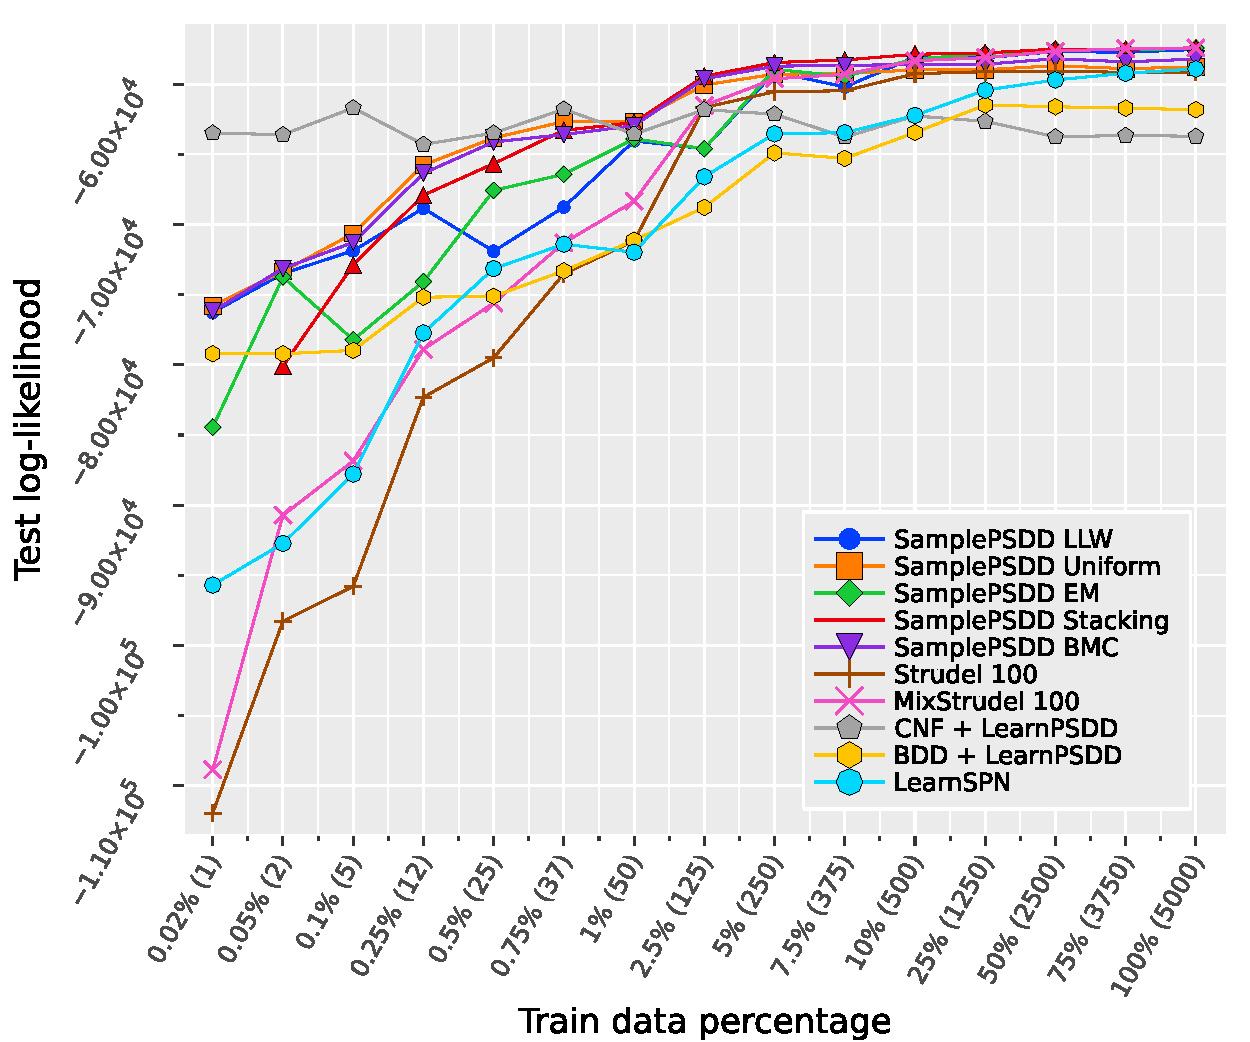
\includegraphics[width=\textwidth]{ll_led}
    \caption{}
    \label{fig:ll-led}
  \end{subfigure}
  \begin{subfigure}{0.495\textwidth}
    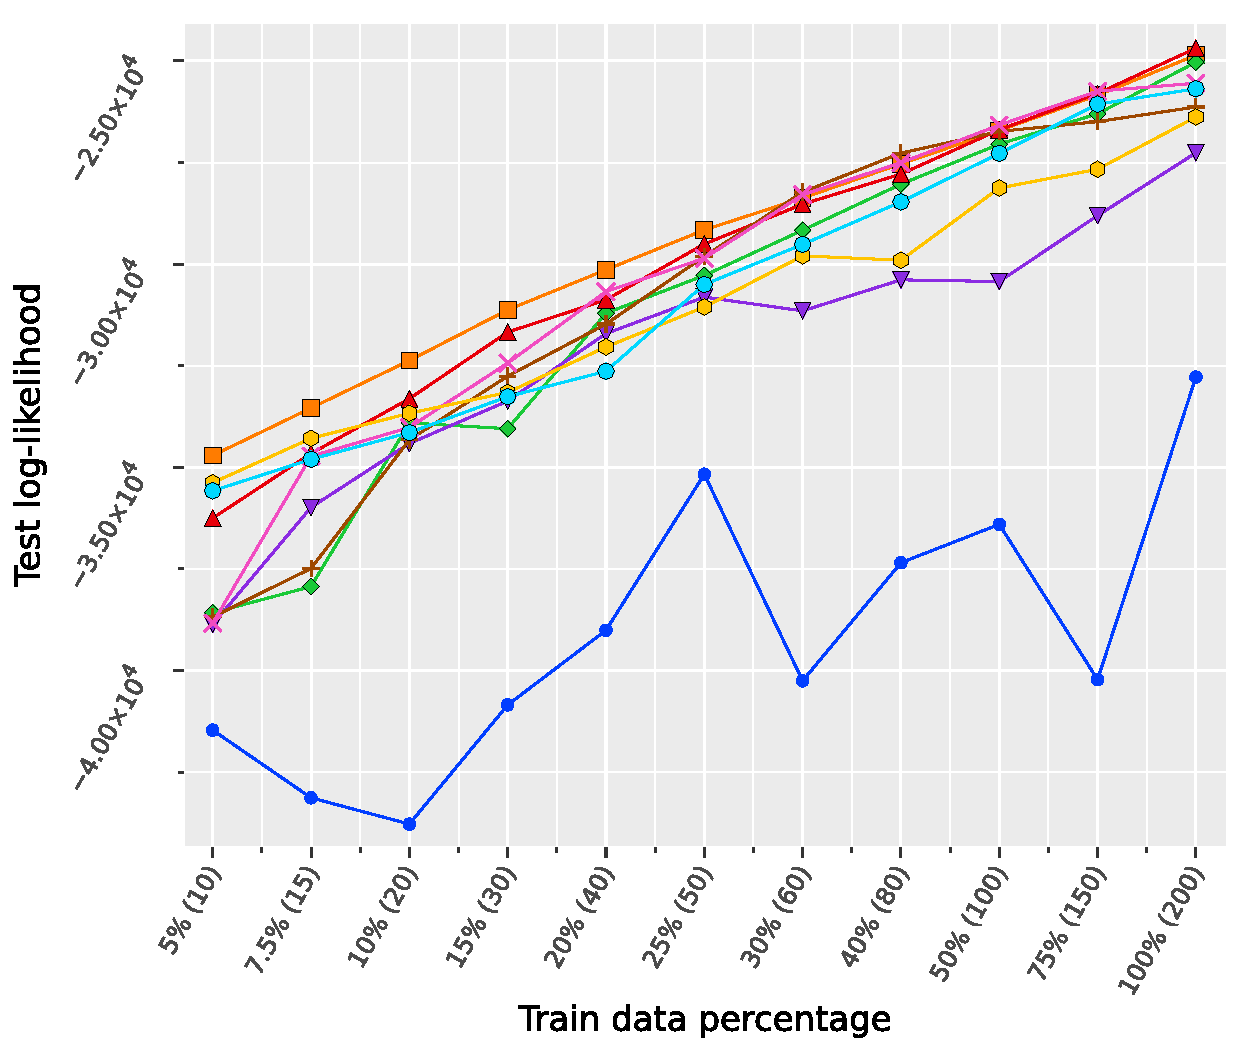
\includegraphics[width=\textwidth]{ll_led_pixels}
    \caption{}
    \label{fig:ll-led-pixels}
  \end{subfigure}
  \caption{Log-likelihoods for the unpixelized \texttt{led} \textbf{(a)} and pixelized
    \texttt{led-pixels} \textbf{(b)} datasets.}
  \label{fig:ll-led-all}
\end{figure}

\Cref{fig:ll-led-all} shows how our approach fairs against competitors using different percentages
of available training data on the unpixelized and pixelized versions of the dataset. The labels on
the $x$-axis indicate percentage and number of training instances. We sampled $t=100$ circuits for
both settings, with $k=32$ and $k=8$ for \texttt{led} and \texttt{led-pixels} respectively. Note
how the use of logical constraints greatly improves performance even under extremely scarce data
(with 1 or 2 datapoints). Most of the \textproc{SamplePSDD} approaches obtain the best performance
with the full dataset, and ranks among the best when data size is small.

\subsubsection{Cardinality Constraints}

The \textproc{dota} dataset contains the result of \num{102944} online matches of the Dota 2
videogame, made available at the UCI Repository. In this game, each team is composed of 5 players
players, with each one controlling a single character out of a pool of 113. Each character can be
controlled by at most one single player in a match. We represent the domain by 2 groups of 113
Boolean variables $C_1^{(i)}$ and $C_2^{(i)}$, denoting whether the $i$-th character was selected
by the first or second team, respectively. We then encode $113$-choose-$5$ cardinality constraints
on the selection of each team (i.e.\ $\sum_{i=1}^113 C_j^{(i)}=5$ for $j\in\{1,2\}$).
Unfortunately, adding the constraint that no character can be selected by both teams
$\neg(C_1^{(i)}\wedge C_2^{(i)})$ made the BDD representation of the formula intractable, and so
was ignored. Since the CNF representation of cardinality constraints is intractable, we used a PSDD
compiled from a BDD to generate an initial circuit for \textproc{LearnPSDD} (as BDDs can
efficiently encode such restrictions \citep{een06}). We set the number of components for
\textproc{SamplePSDD} to $t=30$ and bound the number of sampled elements to $k=3$.

\begin{figure}[t]
  \begin{subfigure}{0.495\textwidth}
    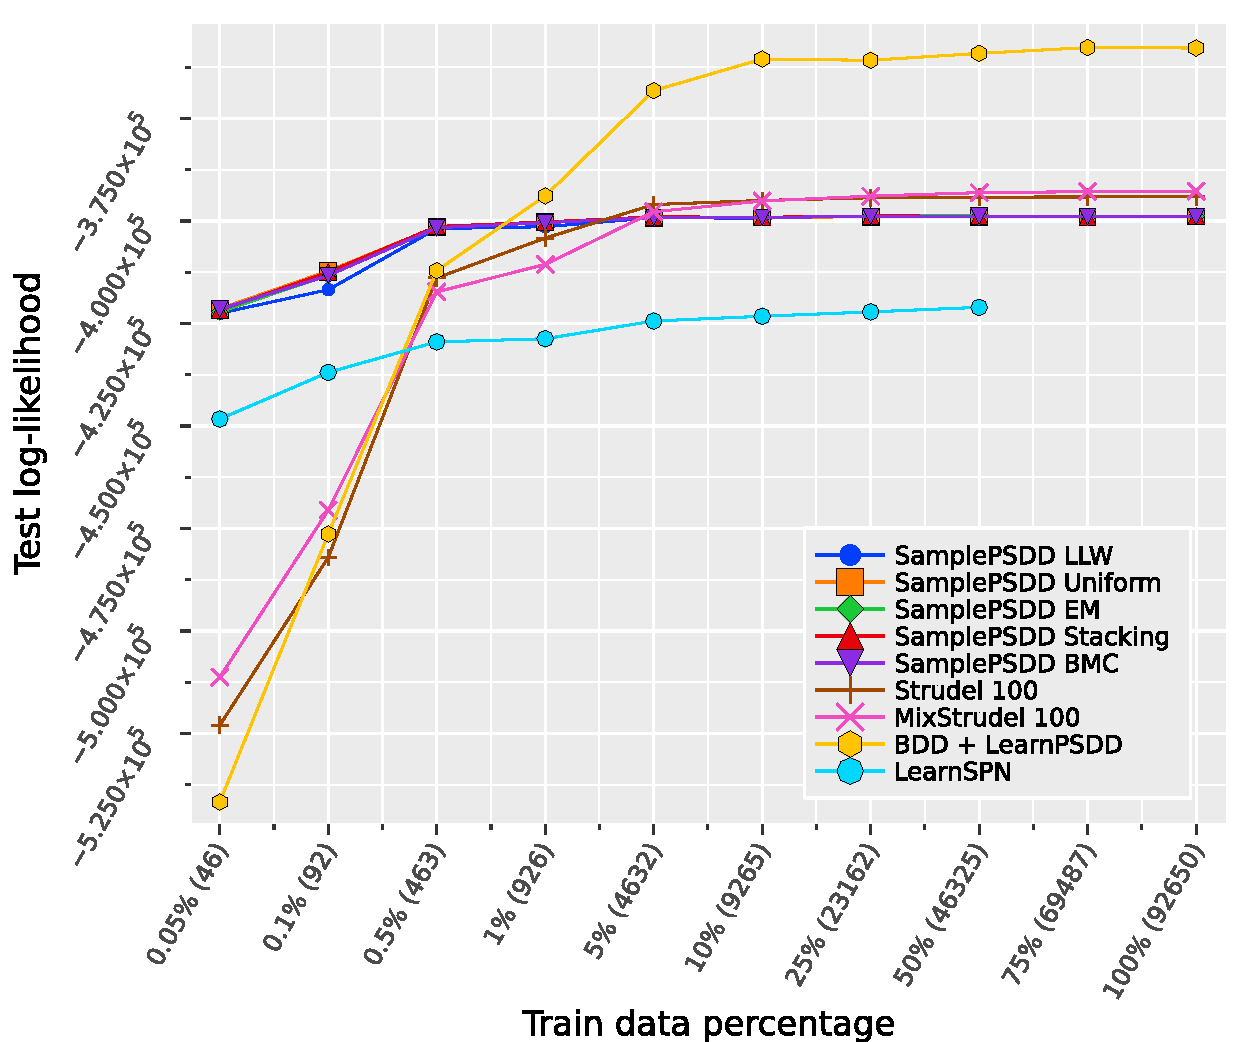
\includegraphics[width=\textwidth]{ll_dota}
    \caption{}
    \label{fig:ll-dota}
  \end{subfigure}
  \begin{subfigure}{0.495\textwidth}
    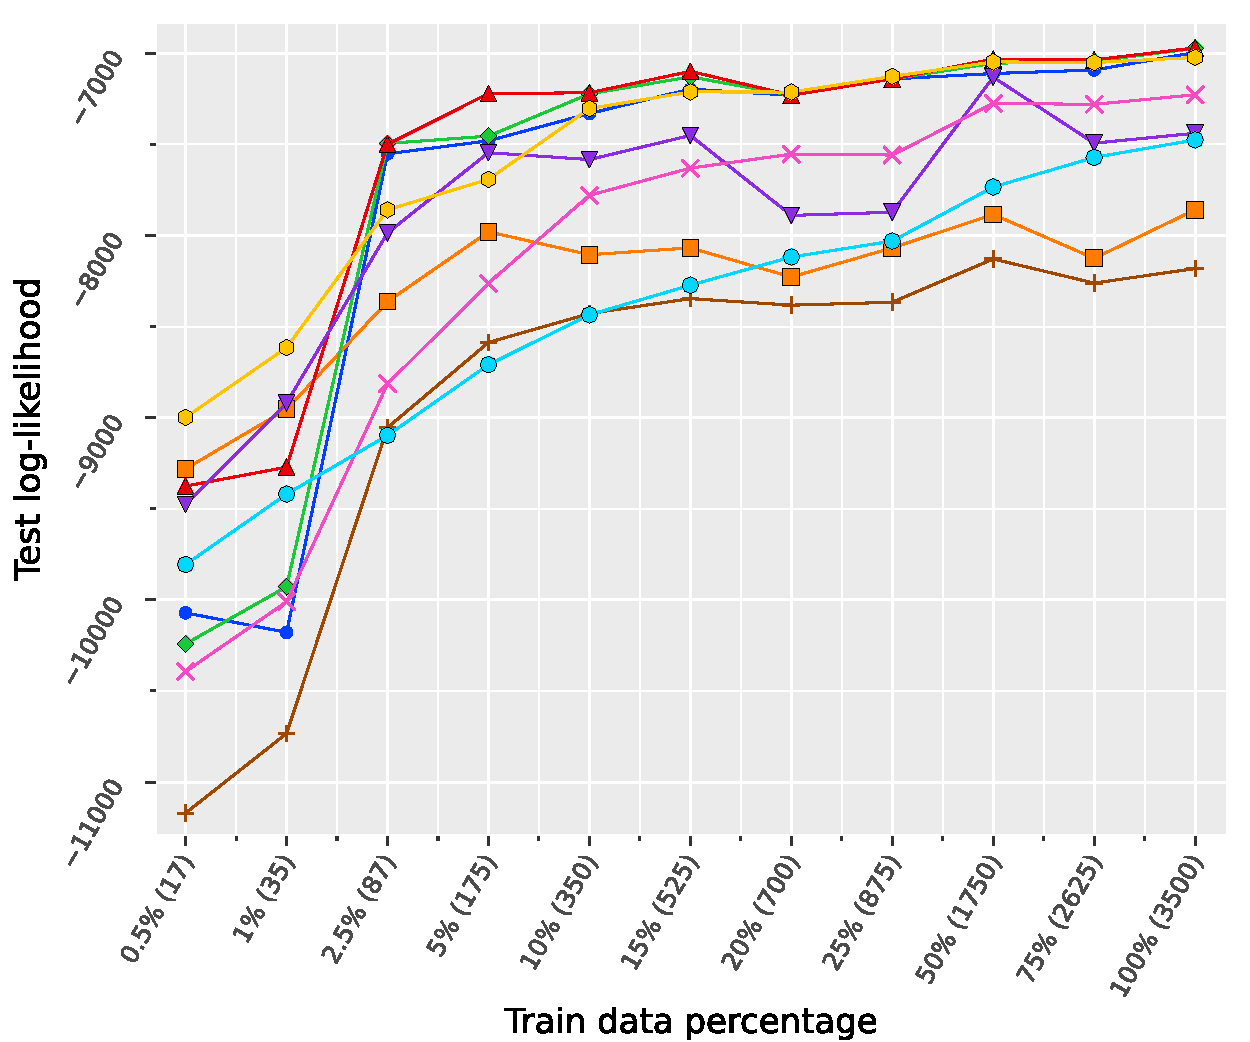
\includegraphics[width=\textwidth]{ll_sushi_choose}
    \caption{}
    \label{fig:ll-sushi-choose}
  \end{subfigure}
  \caption{Log-likelihoods for the \texttt{dota} \textbf{(a)} and $10$-choose-$5$ \texttt{sushi}
    \textbf{(b)} datasets.}
  \label{fig:ll-cardinality}
\end{figure}

The plot in \Cref{fig:ll-dota} shows the test log-likelihood of the tested approaches. Despite
accurately encoding logical constraints, \textproc{LearnPSDD} initially obtains worse performance
when compared to \textproc{SampledPSDD}, but quickly picks up, outperforming other models by a
large margin. \textproc{SamplePSDD} ranks first for small data regimes, and is comparable to
\textproc{Strudel} (and mixtures of) for large training datasets. \textproc{LearnSPN} encountered
problems scaling to more than \num{50000} instances due to intensive memory usage in both
clustering and pairwise independence testing.

We also compared methods on the \texttt{sushi} dataset \citep{kamishima03}, using the setting
proposed in \citet{shen17}. The data contains a collection of \num{5000} rankings of \num{10}
different types of sushi. For each ranking, we create \num{10} Boolean variables denoting whether
an item was ranked among the top 5, and ignore their relative position. The logical constraints
represent the selection of \num{5} out of \num{10} items. We split the dataset into \num{3500}
instances for training and \num{1500} for the test set and evaluated the log-likelihood on both
tasks. The plot in \Cref{fig:ll-sushi-choose} shows the log-likelihood for this data. For this
dataset, we set $t=30$ and $k=3$ for ensembles of \textproc{SamplePSDD}. \textproc{LearPSDD}
obtains superior performance accross some of the low sample sizes, but our approaches were able to
quickly pick up and tie with \textproc{LearnPSDD} when using the LLW, stacking and EM strategies.

\subsubsection{Preference Learning}

We also evaluated performance on the original task of ranking items on the \texttt{sushi} dataset.
We adopt the same encoding and methodology as \citep{choi15}, where each ranking is encoded by a
set of Boolean variables $X_{ij}$ indicating whether the $i$-th item was ranked in the $j$-th
position. We use same parameters for ensembles of \textproc{SamplePSDD} as the previous dataset and
set $t=30$ and $k=3$. The test log-likelihood performance of each different method is shown in
\Cref{fig:ll-sushi-ranking}. The results are qualitatively similar to the previous experiments:
\textproc{SamplePSDD} performed better than pure data approaches under low data yet achieved
competitive results when given the full data. In this case, however, we found that
\textproc{LearnPSDD} ranked first by a large margin compared to others.

\begin{figure}[t]
  \begin{subfigure}{0.495\textwidth}
    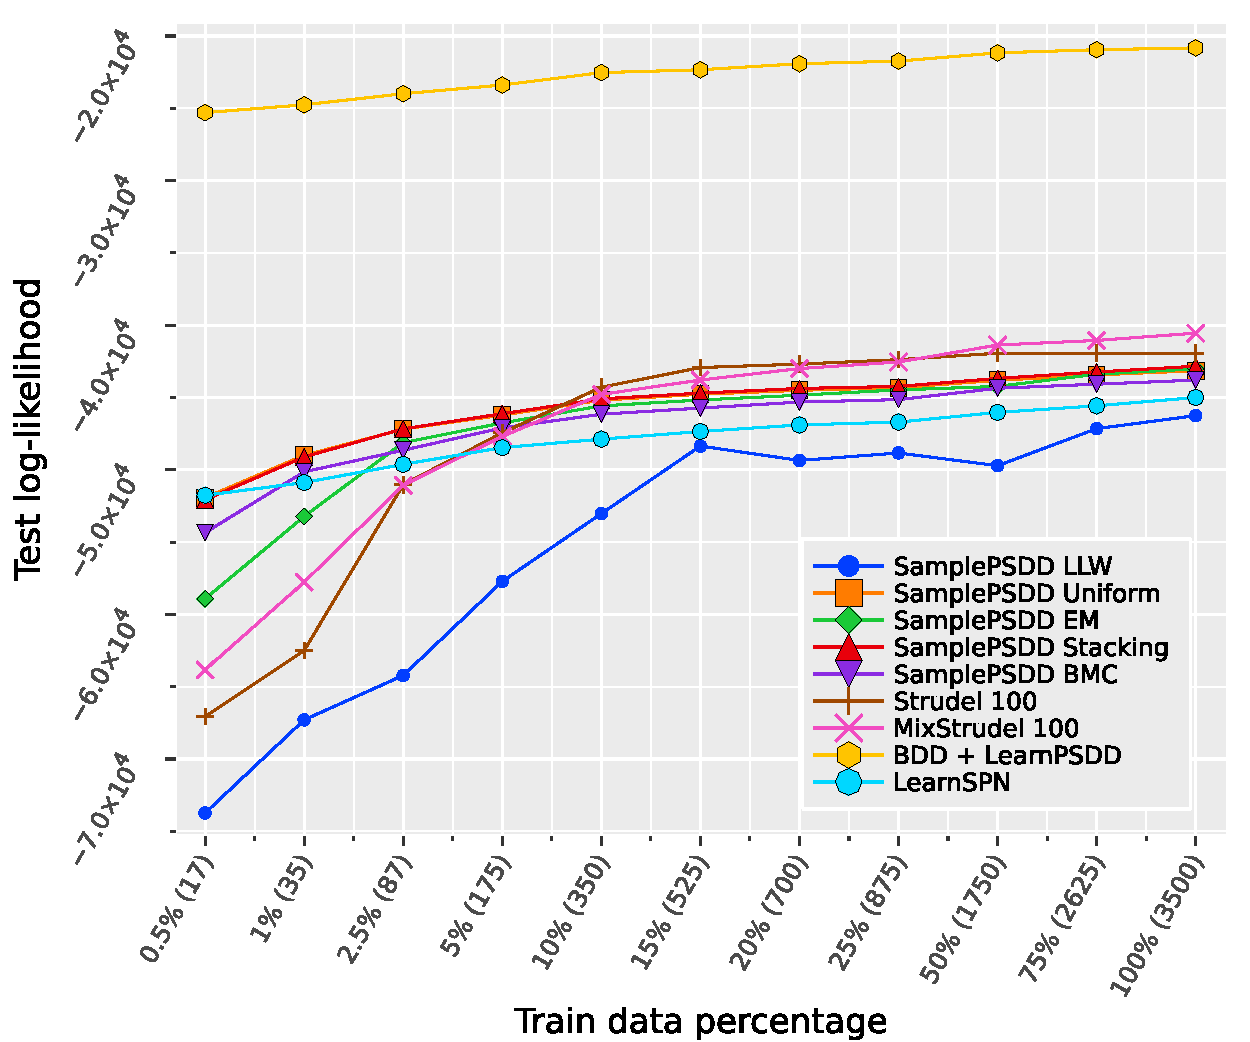
\includegraphics[width=\textwidth]{ll_sushi_ranking}
    \caption{}
    \label{fig:ll-sushi-ranking}
  \end{subfigure}
  \begin{subfigure}{0.495\textwidth}
    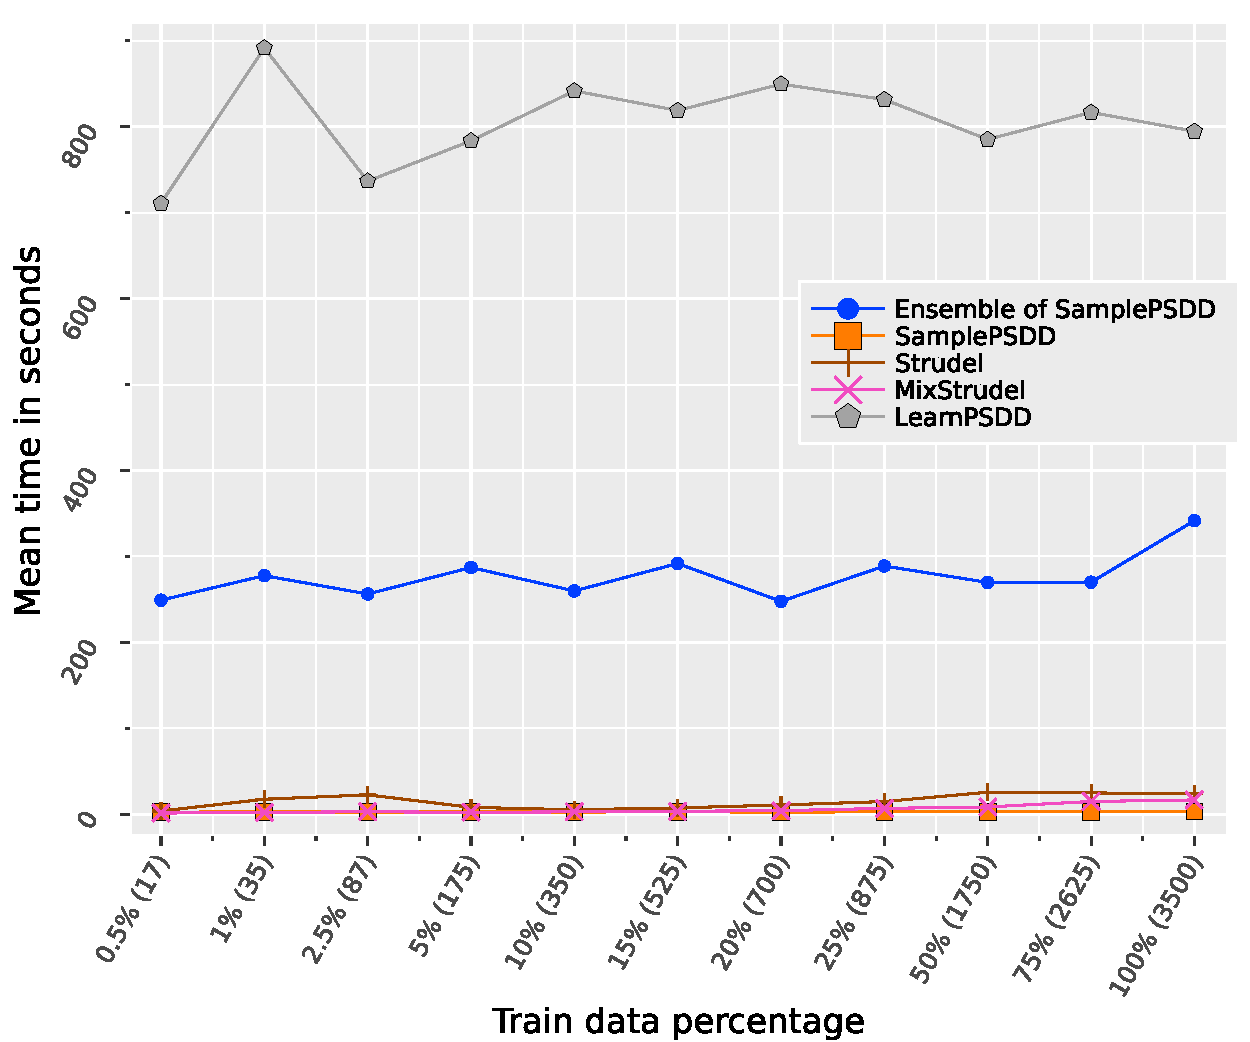
\includegraphics[width=\textwidth]{sushi_time}
    \caption{}
    \label{fig:sushi-time}
  \end{subfigure}
  \caption{Log-likelihood for the \texttt{sushi} ranking \textbf{(a)} dataset and curves for mean
  average time (in seconds) of learning a single \textproc{LearnPSDD} circuit, one
  \textproc{Strudel} circuit (CLT initialized), a mixture of 10 shared-structure \textproc{Strudel}
  components, a single \textproc{SamplePSDD} PC and an ensemble of 100 \textproc{SamplePSDD}
  circuits.}
  \label{fig:ll-preference}
\end{figure}

\subsubsection{Scalability, Complexity and Learning Time}

The major advantage of \textproc{SamplePSDD} compared to other PSDD learning algorithms comes from
its ability to learn from both data and a logical formula $\phi$ even when $\phi$ defines an
intricate Boolean formula over many variables. Interestingly, how capable \textproc{SamplePSDD} is
of learning from $\phi$ comes not only from the algorithm itself, but how $\phi$ is represented. In
fact, any data structure with tractable restriction and reduction (to a canonical form) can be used
in place of the BDD shown in \Cref{alg:samplepsdd}. We do not require forgetting to be tractable
due to an implementational ``trick'' in \textproc{SamplePSDD} that allows a fast implementation to
ignore variables not in the scope of the vtree. More details can be found in the supplemental
material of \Cref{sec:samplepsdd-article}. Consequently, how scalable our proposed algorithm is
depends on the representational power of the tool used for manipulating logical formulae. This is
shown more concretely when we learn from the constraints set by the \texttt{dota} dataset: had we
tried to manipulate formulae with a CNF, the intractability of cardinality constraints would
unfortunately impede any progress.

We no provide an analysis on the complexity of $\textproc{SamplePSDD}$. We start with the
$\textproc{SamplePartialPartition}$ subroutine. If we choose a BDD for manipulating formulae, then
restrictions are done in $\bigo(c\log c)$, where $c$ is the size of the BDD's graph. At every
iteration of the main loop in line \ref{alg:samplepartial:line:while} of \Cref{alg:samplepartial},
a leaf of the binary decision tree is split into two, increasing the number of leaves (and
therefore primes) by one. This is repeated until $k$ leaves of the decision tree have been
expanded, bringing \textproc{SamplePartialPartition}'s complexity to $\bigo(k\cdot c\log c)$. Every
call of \textproc{SamplePSDD} (apart from base cases) produces a new partition and randomly
compress and merge elements. Compression requires applying a disjunction over two primes, both of
which are conjunctions of literals, represented in BDDs as a graph of size linear to the number of
terms. Because primes can have at most $\left\lceil\log_2(k)\right\rceil$, the disjunction of two
such conjunctions is done in $\bigo(\log_2^2 k)$. Merging (or compressing) $n$ elements
essentially subtracts the number of recursive calls for each merge (or compression) by $n-1$.
Therefore, every \textproc{SamplePSDD} recursive call is $\bigo\left(k\cdot c\log c+\log_2^2 k
\right)$.

We empirically evaluate the time it takes to learn a single circuit from each of
\textproc{LearnPSDD}, \textproc{Strudel} and \textproc{SamplePSDD}. We also measure running times
for learning 10 structure-sharing circuits as components of a mixture of \textproc{Strudel}s and
100 (structurally) distinct PCs sampled from \textproc{SamplePSDD}, each with parameters learned
from closed-form MLE. \Cref{fig:sushi-time} shows the time it takes to run each of these settings
on the \texttt{sushi} ranking dataset. On average, \textproc{Strudel} took approximately \num{15}
seconds, \textproc{LearnPSDD} \num{13} minutes and \num{25} seconds, and \textproc{SamplePSDD}
about \num{2.76} seconds for learning a single PSDD.

\subsubsection{Performance and Sampling Bias}

The approximation quality of \textproc{SamplePSDD} is highly dependent on both the vtree and
maximum number of primes. In this section, we compare the impact of both in terms of performance
and circuit complexity. We assess performance by the log-likelihoods in the test set, as well as
consistency with the original logical constraints. The latter is measured by randomly sampling
\num{5000} (possibly invalid) instances and evaluating whether the circuit correctly decides their
value. A set of the top \num{100} sampled PSDDs (in terms of log-likelihood in the train set) are
selected out of \num{500} circuits learned on the $10$-choose-$5$ \texttt{sushi} dataset to compose
the ensemble. Circuit complexity is estimated in terms of both time taken to sample all 500
circuits and graph size (i.e.\ number of nodes) of each individually generated PSDD.

\begin{figure}[t]
  \begin{subfigure}{0.495\textwidth}
    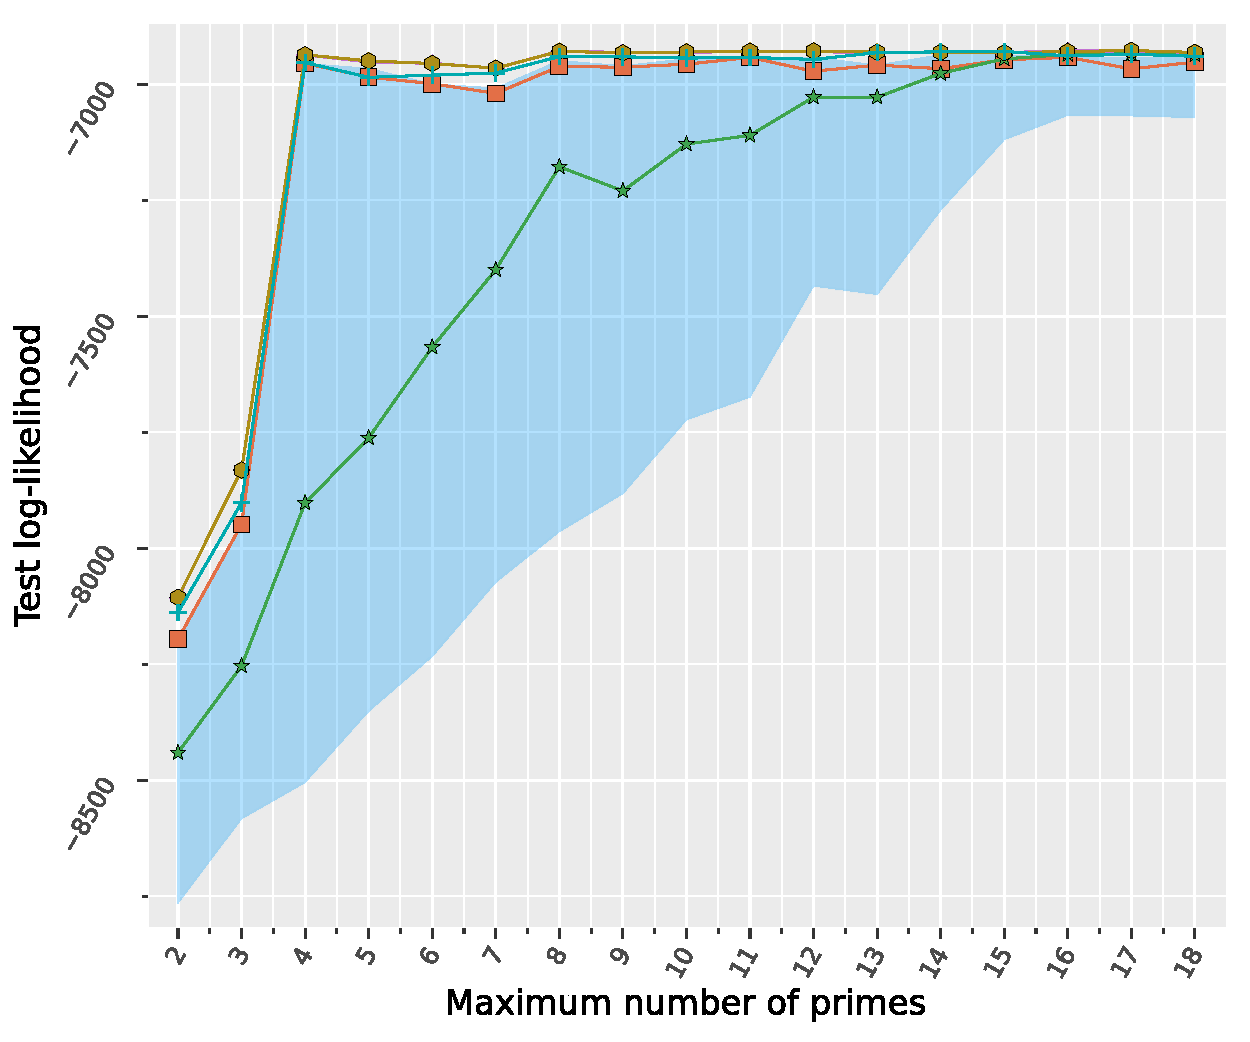
\includegraphics[width=\textwidth]{k_ll}
    \caption{}
  \end{subfigure}
  \begin{subfigure}{0.495\textwidth}
    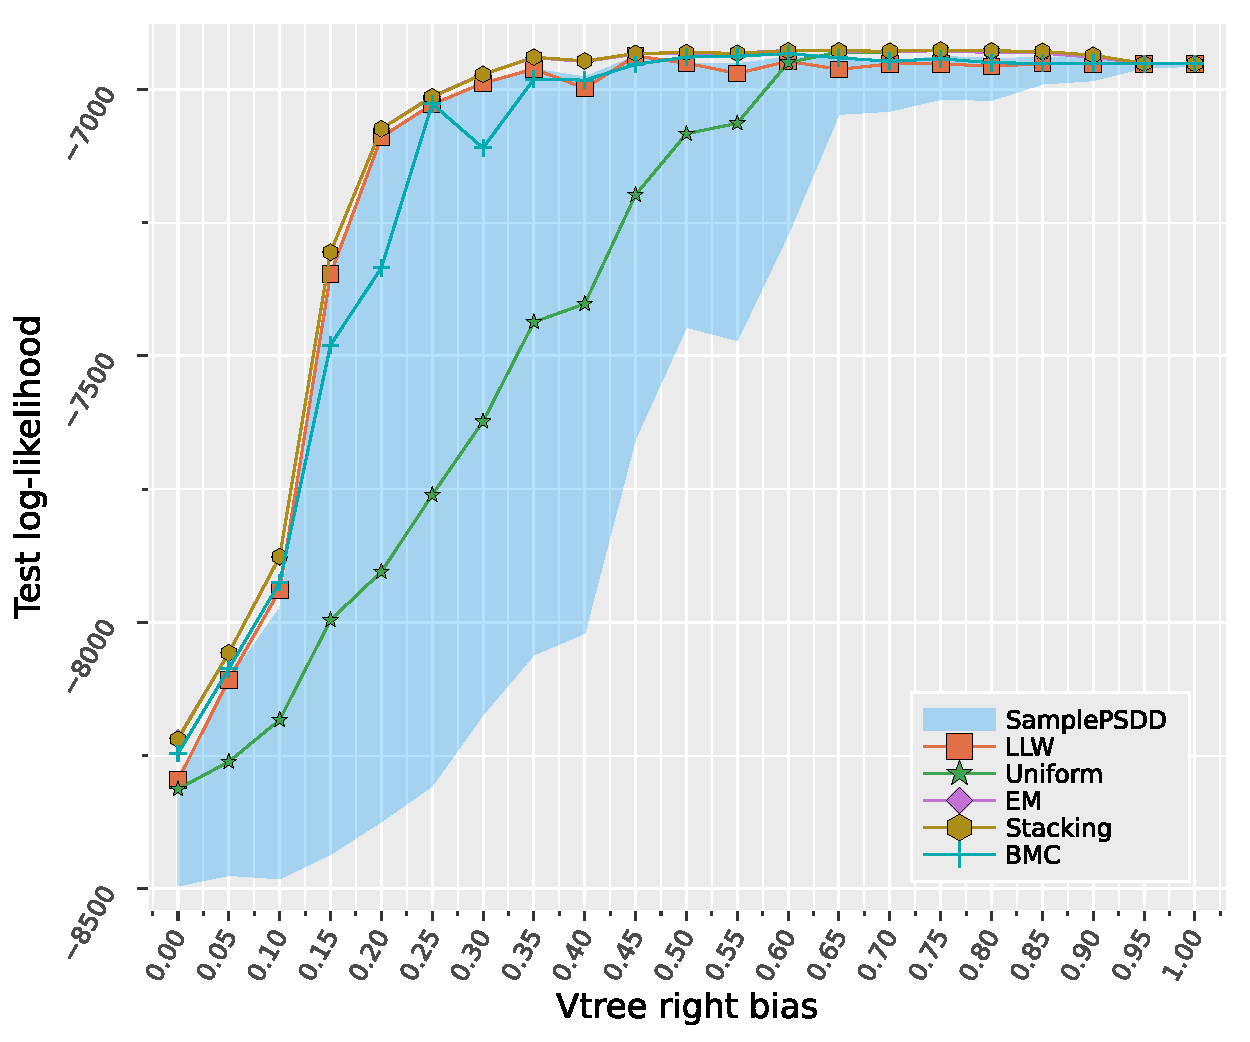
\includegraphics[width=\textwidth]{vtree_ll}
    \caption{}
  \end{subfigure}
  \caption{Impact of the number of bounded primes (left) and structure of vtree (right) on the
    test log-likelihood for the $10$-choose-$5$ \texttt{sushi} dataset.}
  \label{fig:ll-comp}
\end{figure}

It is quite clear that the structure of the vtree is tightly linked to the structure of a PSDD,
especially given the graphical constraints imposed by \textproc{SamplePSDD} and the fact that subs
need to obey a vtree's scope (and thus its structure). For instance, (near) right vtrees keep the
number of primes fixed and require no approximation, while (near) left vtrees discard a large
number of primes. In order to evaluate the effect of the type of vtree on the quality of sampled
structures, we compared the performance of \textsc{SamplePSDD} as we vary the bias towards
generation of right-leaning vtrees. Given a parameter $p$, we grow a vtree in a top-down manner
where at each node we independently assign each variable to the right child with probability $p$.
Small values of $p$ produce left-leaning vtrees, while vtrees are more likely to lean to the
right when $p>0.5$. Left leaning vtrees produce especially small networks compared to other vtrees,
as more variables are left unmentioned because of relaxations coming from the need for a bounded
number of primes. To produce decently sized circuits, we increase the number of sampled primes $k$
when $p$ is low and decrease $k$ when $p$ is high.

\Cref{fig:ll-comp} shows the log-likelihood, \Cref{fig:imp-comp} shows consistency and
\Cref{fig:compl-comp} shows circuit complexity when varying the type of vtrees (left) used for
guiding the PSDD construction and the bound on the number of primes (right). The blue shaded area
represents the interval of values (worse to best ranked) for individual circuits. To verify
consistency, we evaluate the PSDDs in terms of satisfiability of a given example. An ensemble
returned a configuration as satisfiable if any of its models attributed some nonzero probability to
it; and unsatisfiable if all models gave zero probability. This evaluation gives a lower bound to
consistency, which means all models eventually unanimously agreed on satisfiability when vtree
right bias $\geq 0.65$. Alternatively, since \textproc{SamplePSDD} is a relaxation of the original
formula, an upper bound on consistency could be achieved by evaluating whether any model within the
ensemble gave a zero probability to the example; this upper bound curve on consistency would be
equivalent to the top side of the shaded area. Interestingly, we note that the likelihood weighting
strategy (LLW) dominates over others on consistency. This is because LLW often degenerates to a few
models, giving zero probability to lower scoring PSDDs, which means only a small subset of circuits
decide on satisfiability, and thus a more relaxed model is less likely to disagree with the
consensus. On the other hand, this does not translate to better data fitness on the general case,
as we clearly see in \Cref{fig:ll-led-all,fig:ll-cardinality,fig:ll-preference}.


\begin{figure}[t]
  \begin{subfigure}{0.495\textwidth}
    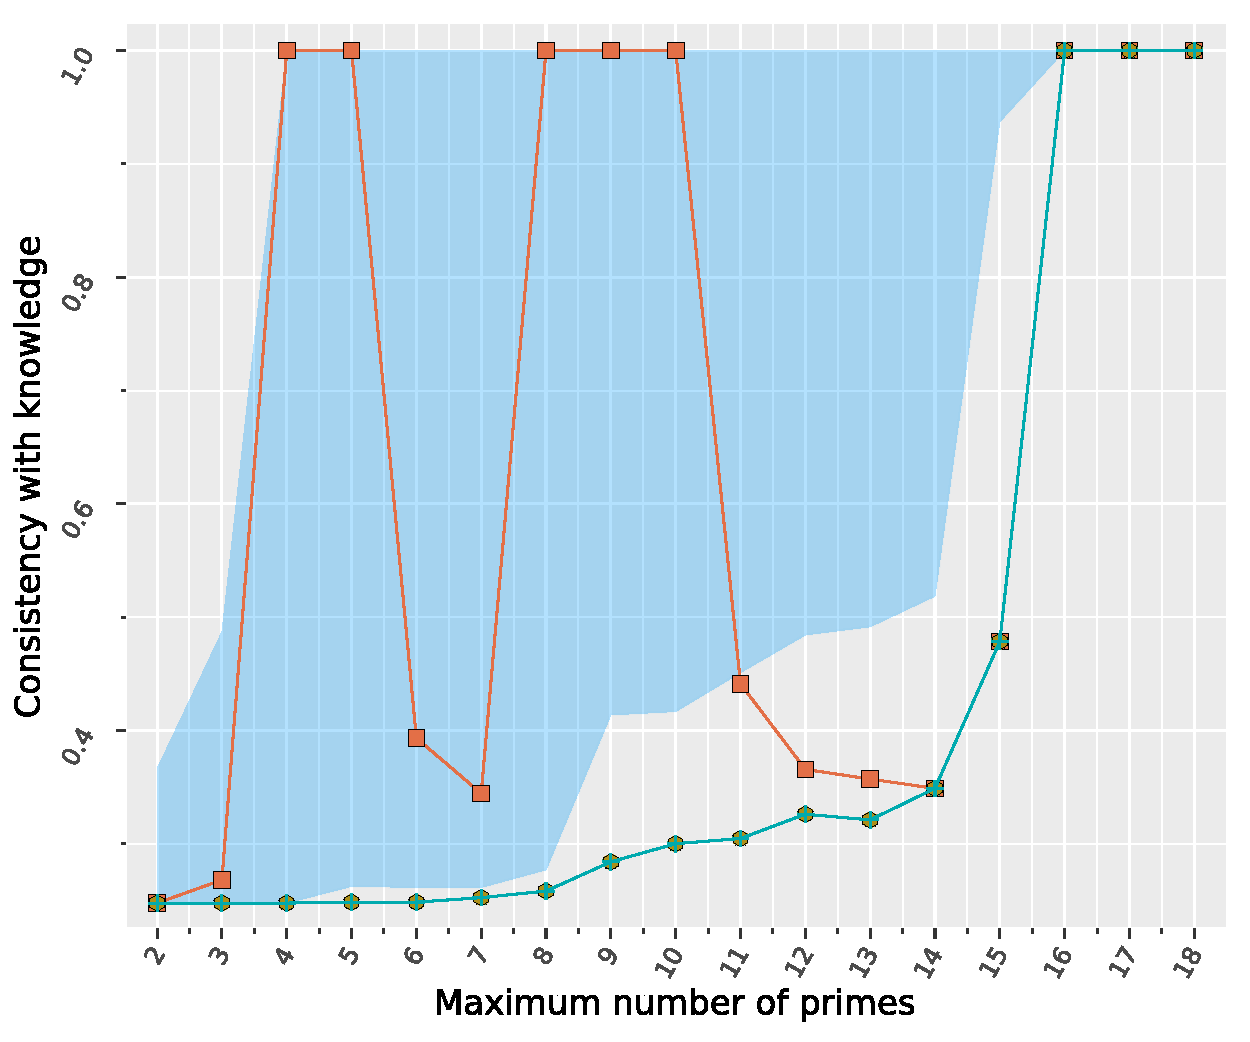
\includegraphics[width=\textwidth]{k_imp}
    \caption{}
  \end{subfigure}
  \begin{subfigure}{0.495\textwidth}
    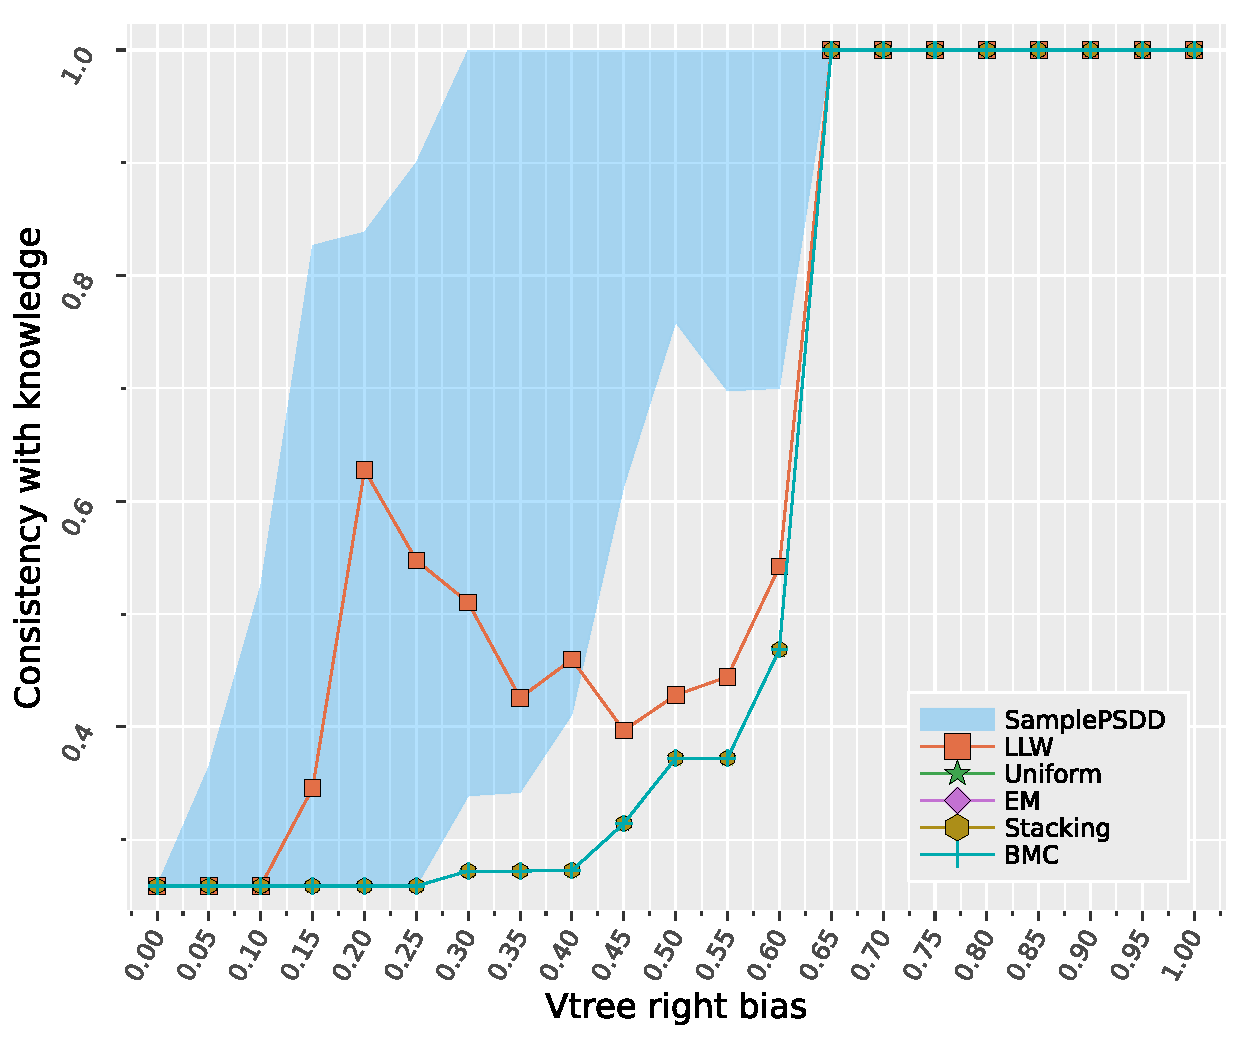
\includegraphics[width=\textwidth]{vtree_imp}
    \caption{}
  \end{subfigure}
  \caption{Impact of the number of bounded primes (left) and structure of vtree (right) on the
    consistency of sampled PSDDs with the original logical constraints for the $10$-choose-$5$
    \texttt{sushi} dataset.}
  \label{fig:imp-comp}
\end{figure}

\begin{figure}[t]
  \begin{subfigure}{0.495\textwidth}
    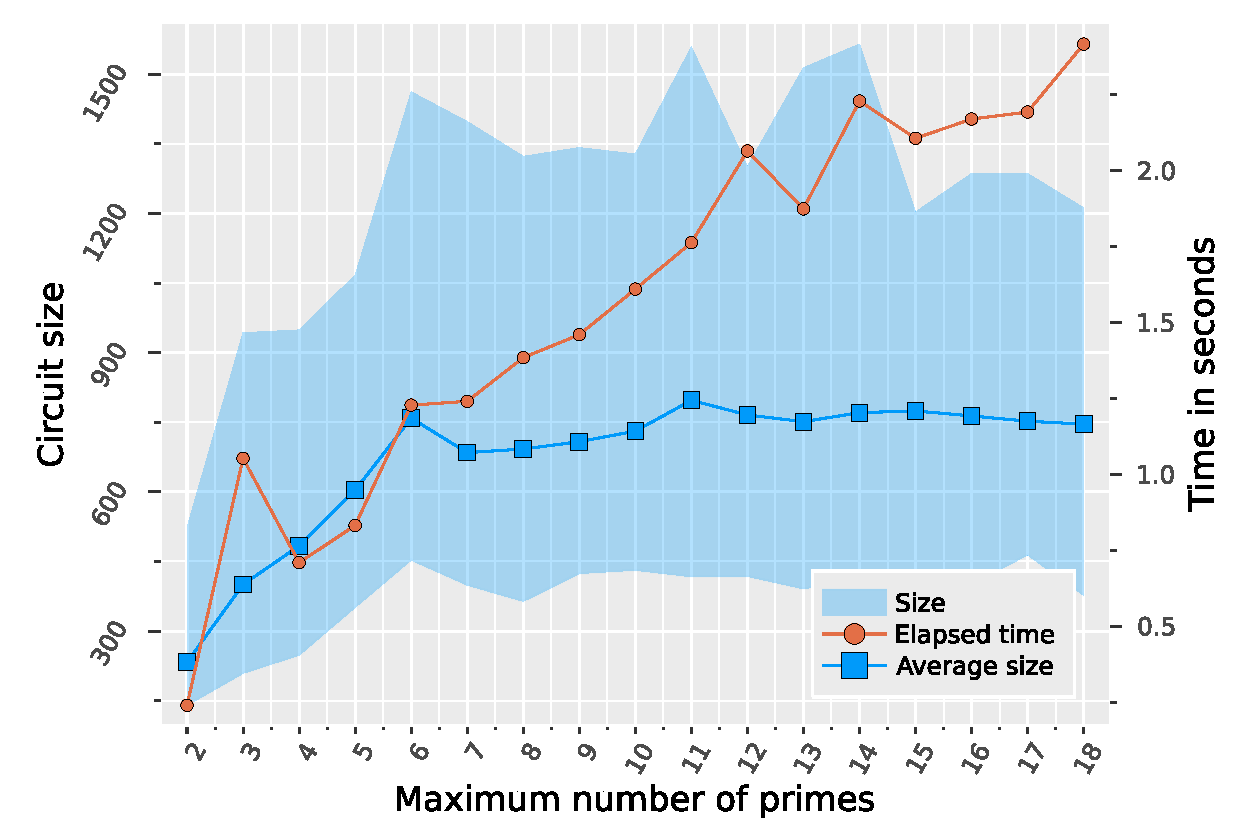
\includegraphics[width=\textwidth]{k_complexity}
    \caption{}
  \end{subfigure}
  \begin{subfigure}{0.495\textwidth}
    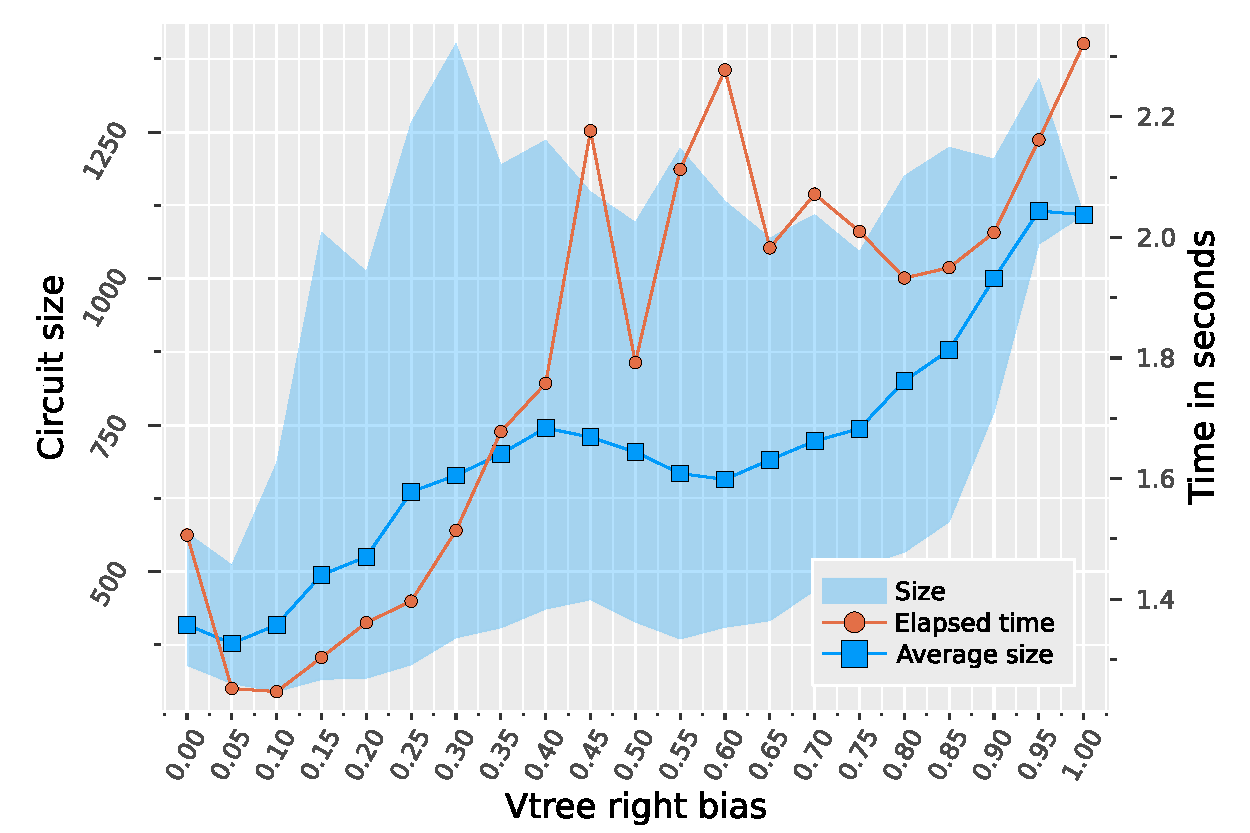
\includegraphics[width=\textwidth]{vtree_complexity}
    \caption{}
  \end{subfigure}
  \caption{Impact of the number of bounded primes (left) and structure of vtree (right) on circuit
    size (in number of nodes) and learning time (in seconds) for the $10$-choose-$5$ \texttt{sushi}
    dataset.}
  \label{fig:compl-comp}
\end{figure}

\section{A Data Perspective}
\label{sec:data}

\subsection{\textproc{LearnRP}}

\subsection{Experiments}
